\documentclass[12pt,a4paper]{article}
\usepackage[utf8]{inputenc}
\usepackage{amsfonts}
\usepackage{amssymb}
\usepackage{amsmath}
\usepackage{graphicx}
\usepackage{float}

% sets margin
\usepackage[hmargin=3cm,vmargin=2.5cm]{geometry}

% creates landscape pages
\usepackage{pdflscape}
\usepackage{pdfpages}

%\renewcommand{\rmdefault}{phv} % Arial
\renewcommand{\sfdefault}{phv} % Arial

% defining settings for textpos
\usepackage[absolute]{textpos}
\setlength{\TPHorizModule}{\paperwidth}
\setlength{\TPVertModule}{\paperheight}

% headers / footers
\usepackage{fancyhdr}
\pagestyle{fancy}
\fancyhf{}
\rhead{Assignment 1B}
\lhead{CSG2341: Intelligent Systems}
\rfoot{\thepage}
\lfoot{Martin Ponce, ID: 10371381}
\renewcommand{\footrulewidth}{0.5pt}

% defining landscape headers / footers
\fancypagestyle{fancylscape}{
	\fancyhf{}
	\renewcommand{\footrulewidth}{0pt}
	\renewcommand{\headrulewidth}{0pt}
	% header
	\begin{textblock}{0.05}[-0.5,-2](0,0)
		{\rotatebox{90}{CSG2341: Intelligent Systems}}
	\end{textblock}
		\begin{textblock}{0.05}[-0.5,-1](0,0)
		{\rotatebox{90}{Assignment 1B}}
	\end{textblock}
	\begin{textblock}{0.05}[-1,-0.109](0,0)
		{\rotatebox{90}{\rule{24.2cm}{0.5pt}}}
	\end{textblock}
	% footer
	\begin{textblock}{0.05}[-19,-4.28](0,0)
		{\rotatebox{90}{Martin Ponce, ID: 10371381}}
	\end{textblock}
		\begin{textblock}{0.05}[-19,-12.8](0,0)
		{\rotatebox{90}{\thepage}}
	\end{textblock}
		\begin{textblock}{0.05}[-18.7,-0.109](0,0)
		{\rotatebox{90}{\rule{24.2cm}{0.5pt}}}
	\end{textblock}
}

% adjusts padding between caption and figure
\setlength{\belowcaptionskip}{10pt}

% adds links to references and colors them blue
\usepackage{hyperref}
\hypersetup{colorlinks=true,
			linkcolor=blue,
			citecolor=black,
			urlcolor=blue}

% apa style referencing
\usepackage[sectionbib, natbibapa]{apacite}
\usepackage{chbibref}

% underlining text
\usepackage[normalem]{ulem}

% \citetapos for possesive citations
\newcommand{\citetapos}[1]{\citeauthor{#1}{\textcolor{black}{'s}} \citeyearpar{#1}}

% add multiline comments \begin{comment} \end{comment}
\usepackage{verbatim}

% add minted package for code highlighting, number per section
\usepackage[section]{minted}

% add tcolorbox package to style code
\usepackage{tcolorbox}
\tcbuselibrary{minted,skins}

% javacode style config
\newtcblisting{javacode}{
  listing engine=minted,
  colback=bg,
  colframe=black!80,
  listing only,
  minted style=monokai,
  minted language=java,
  minted options={linenos=true,texcl=true,fontsize=\scriptsize},
  left=1mm,
}

% consolecode style config
\newtcblisting{consolecode}{
  listing engine=minted,
  colback=bg,
  colframe=black!80,
  listing only,
  minted style=vim,
  minted language=console,
  minted options={texcl=true,fontsize=\scriptsize},
  left=1mm,
}

% define bg color for code highlighting
\definecolor{bg}{rgb}{0.20,0.20,0.20}

% listings package
\usepackage{listings}
% change label to code
\renewcommand\listingscaption{Java code}

% modify enumerate sub list
\renewcommand{\labelenumii}{\theenumii}
\renewcommand{\theenumii}{\theenumi.\arabic{enumii}.}
\renewcommand{\theenumiii}{\theenumii\arabic{enumiii}}
\renewcommand{\theenumiv}{\theenumiii.\arabic{enumiv}}

% number each equation per section
\numberwithin{equation}{section}

% tikz graphics package
\usepackage{tikz}
\usetikzlibrary{arrows,positioning, calc}
\tikzstyle{vertex}=[draw,fill=black!15,circle,minimum size=18pt,inner sep=0pt]

% environ package, used for larger equations
\usepackage{environ}
\NewEnviron{lequation}{%
    \begin{equation}
    \scalebox{2}{$\BODY$}
    \end{equation}
}

% front matter
\title{Edith Cowan University
\\\leavevmode\\CSG2341\\Intelligent Systems
\\\leavevmode\\Assignment 1B
\\\leavevmode\\Saucers Part 2}
\author{Martin Ponce\\Student 10371381\\\\Tutor: Philip Hingston}
\date{\today}

\begin{document}

% title page
\newpage
\null  % Empty line
\nointerlineskip  % No skip for prev line
\vfill
\let\snewpage \newpage
\let\newpage \relax
\maketitle
\thispagestyle{empty}
\let \newpage \snewpage
\vfill

% toc
\newpage
\tableofcontents
\thispagestyle{fancy}

\newpage
\section{Introduction}

The Board of Directors at Blue Ink have recently become aware of the lack of computer security awareness and best practices amongst its employees. As a result, Blue Ink have requested that a sample Virtual Machine (VM) image of a typical computer within their organisation be analysed for security issues.

This report outlines the security issues identified during the analysis of Blue Ink's sample VM image. Vulnerabilities have been found with the operating system itself, and support software packaged with the operating system, such as the Internet browser and anti-virus application. Vulnerabilities have also been identified in outdated software whilst practices regarding the storage of passwords in plain-text files within user documents folders provide opportunities for unwanted access. The security issues identified in this report must be addressed in order to maintain the utmost security.

\subsection{Assumptions}

\begin{itemize}
\item A firewall is implemented within the network
\end{itemize}

\section{Idea}

The main tactic for this controller is fly defensively in order to conserve energy and survive until there are a two enemies left. Turns for the most part will focus on the energy blast sensor, in order to dodge as many of them as possible. When there are only two enemy saucers left in the arena, turning will focus on the enemy saucer sensor, to track them down and shoot at them from a close distance.

However, when any power ups spawn nearby, the goal is to move straight to the power up, ignoring any energy blasts. If any close energy blasts close to the player while attempting to retrieve a power up, the player will raise the shield. The rate of fire will be kept to a minimum for most situations to conserve energy, unless a nearby power up spawns, or if there is only two remaining enemy saucers left. In these cases, the rate of fire will increase, to either deter enemy saucers from retrieving the power up, or attempt to destroy them.

Speed will also be kept at the minimum for most situations, only increasing speed when necessary for dodging, or when a power up spawns nearby, to try and get to it first. Speed will also be increased when there are only two remaining enemy saucers left, attempting to destroy them before the timer runs out.

This controller attempts to implement these strategies with turning, speed, shields and firepower, with the primary goal of flying defensively by dodging energy blasts and retrieving nearby power ups. When there are only two enemies left, the saucer will begin to fly offensively, increasing speed and firepower, and attempt to destroy the enemies before the timer runs out.
\section{Input linguistic variables}

\subsection{myEnergy}

The linguistic variable \emph{myEnergy} is the player's energy level and determines whether or not the player has \emph{lowEnergy} or \emph{highEnergy} remaining. The universe of disclosure for \emph{myEnergy} is between 0 joules and 10,000 joules, the amount of energy that all saucers begin with.

\begin{figure}[H]
\centering
\caption{\emph{myEnergy} fuzzy sets}
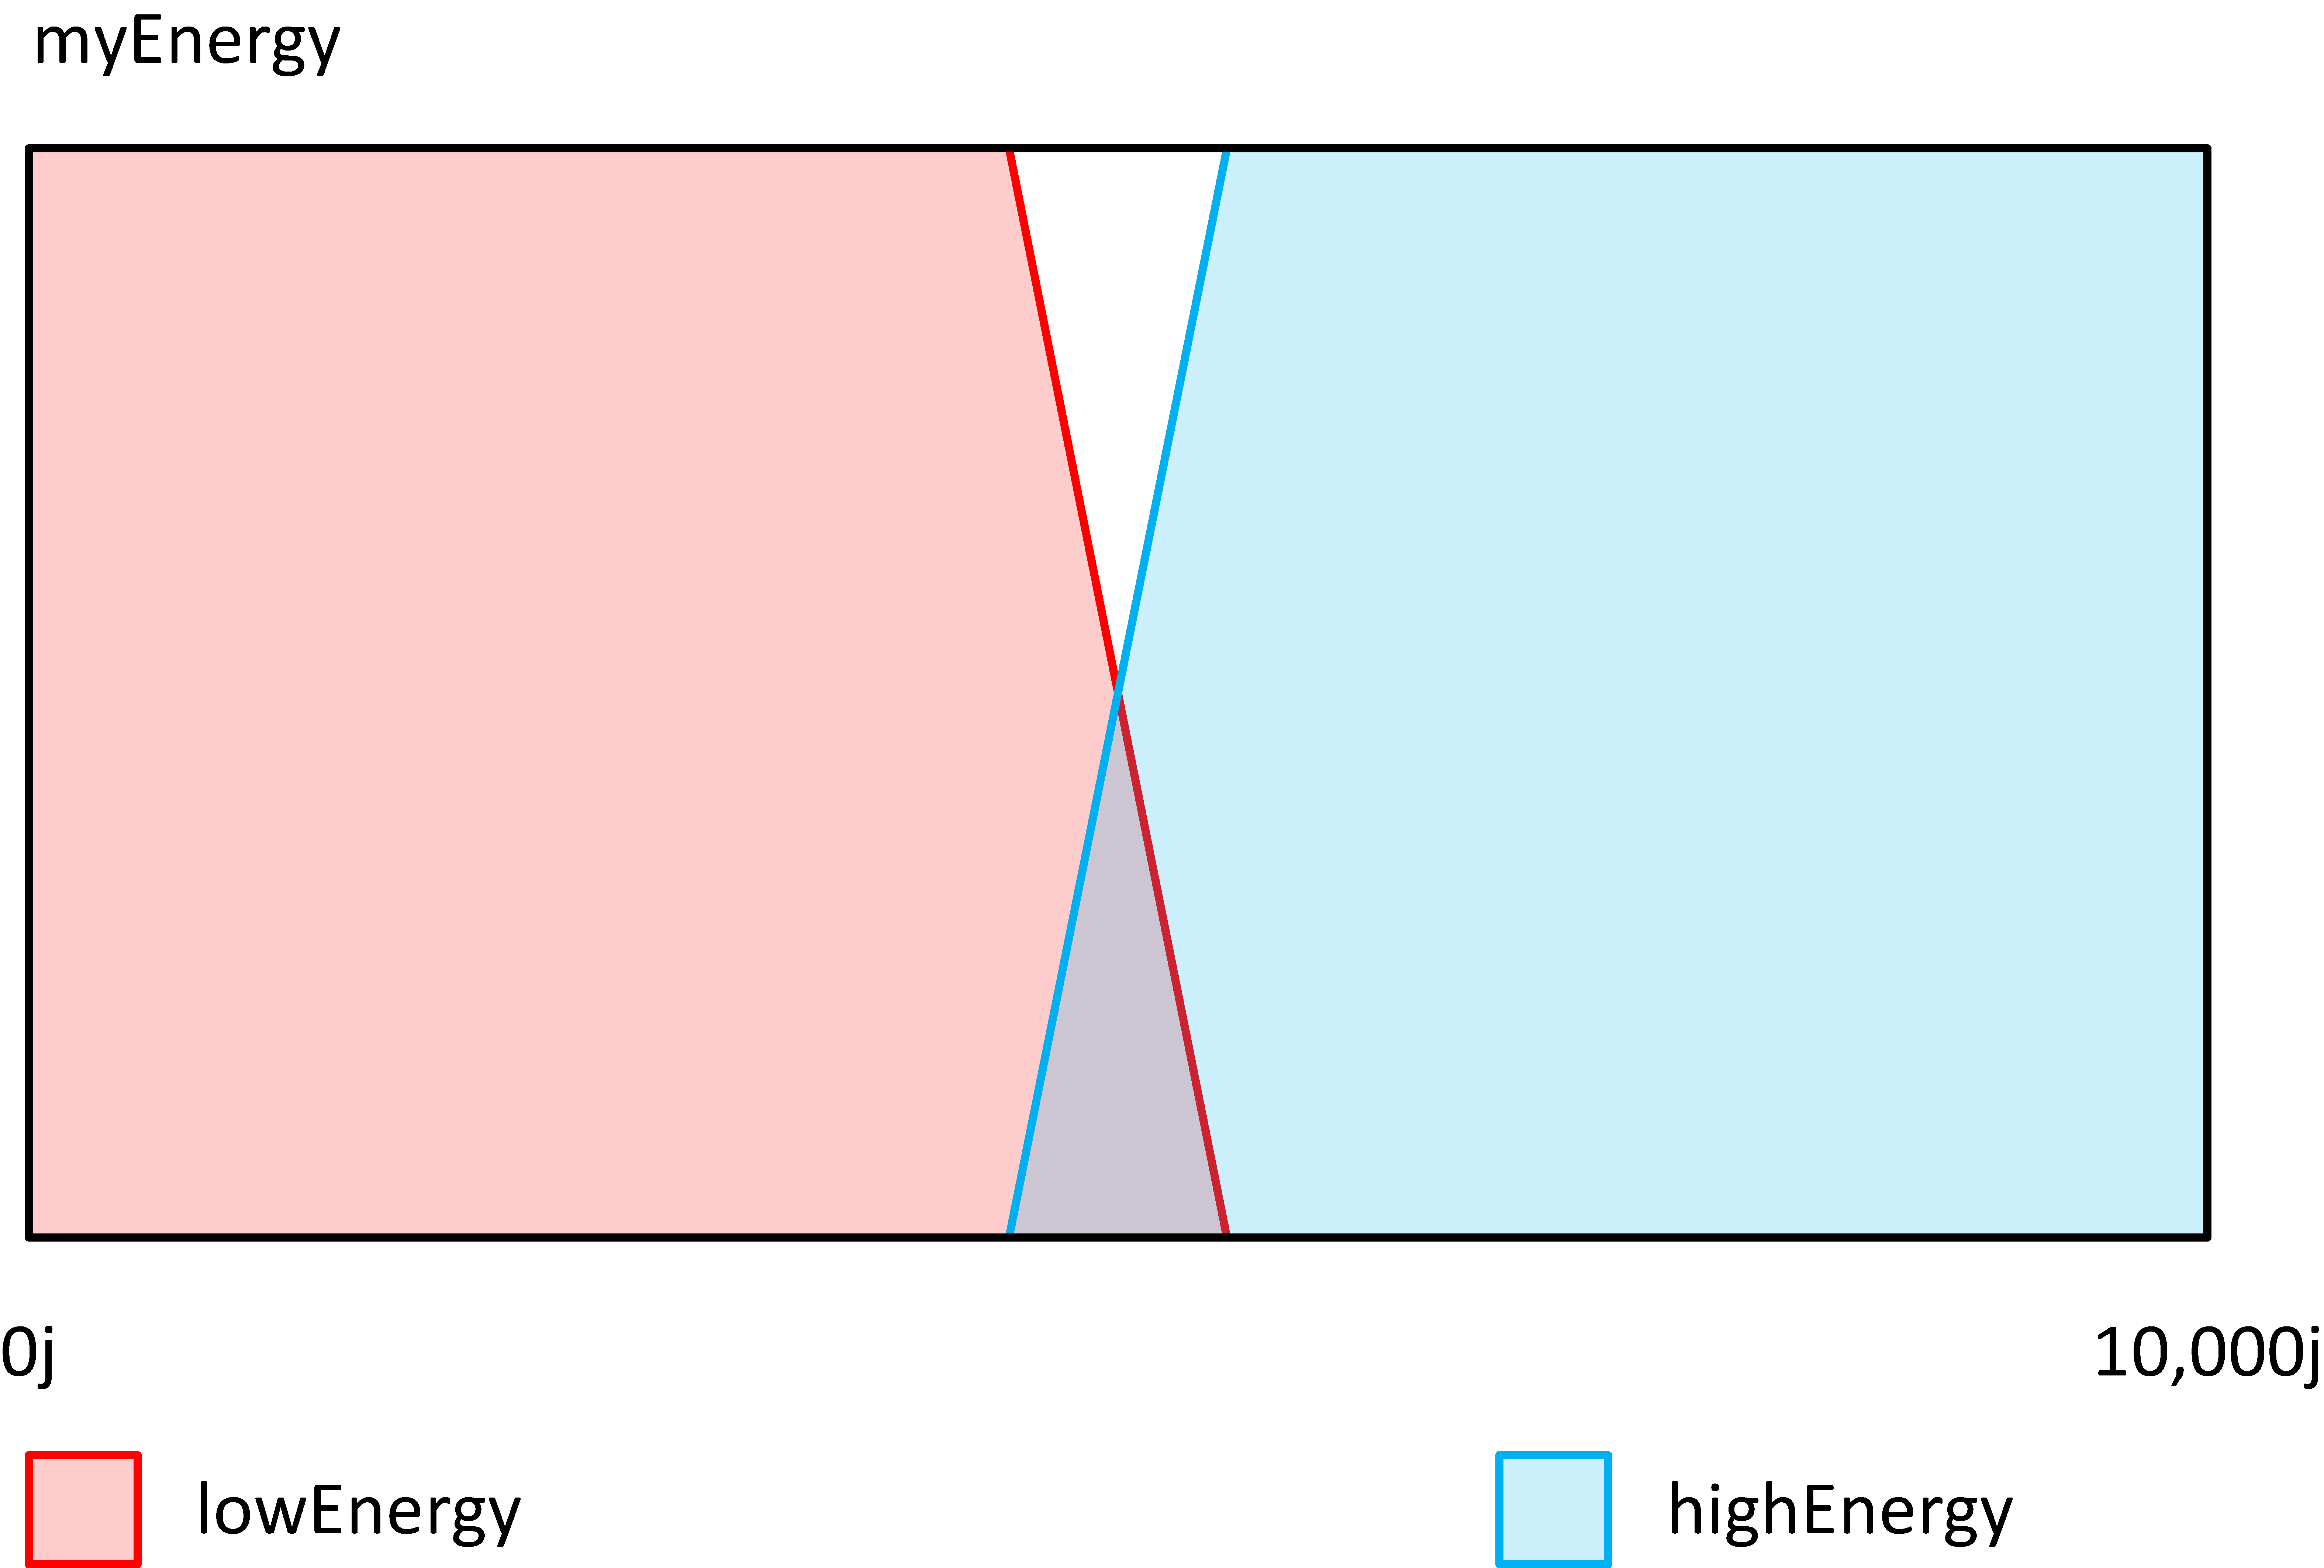
\includegraphics[scale=0.08]{./img/pdf/myEnergySets.pdf}
\end{figure}

\subsection{Target variables}

The sensor returns a list of all the enemy saucers currently in the battle space. This controller only considers the closest saucer as the target, and ignores all other saucers in the list.

\subsubsection{targetDist}

The linguistic variable \emph{targetDist} is the distance from the player to the target. The universe of disclosure for \emph{targetDist} is between 0m and 4802.3m, and the fuzzy sets are defined as \emph{close}, \emph{near}, and \emph{far}.

\begin{figure}[H]
\centering
\caption{\emph{targetDist} fuzzy sets}
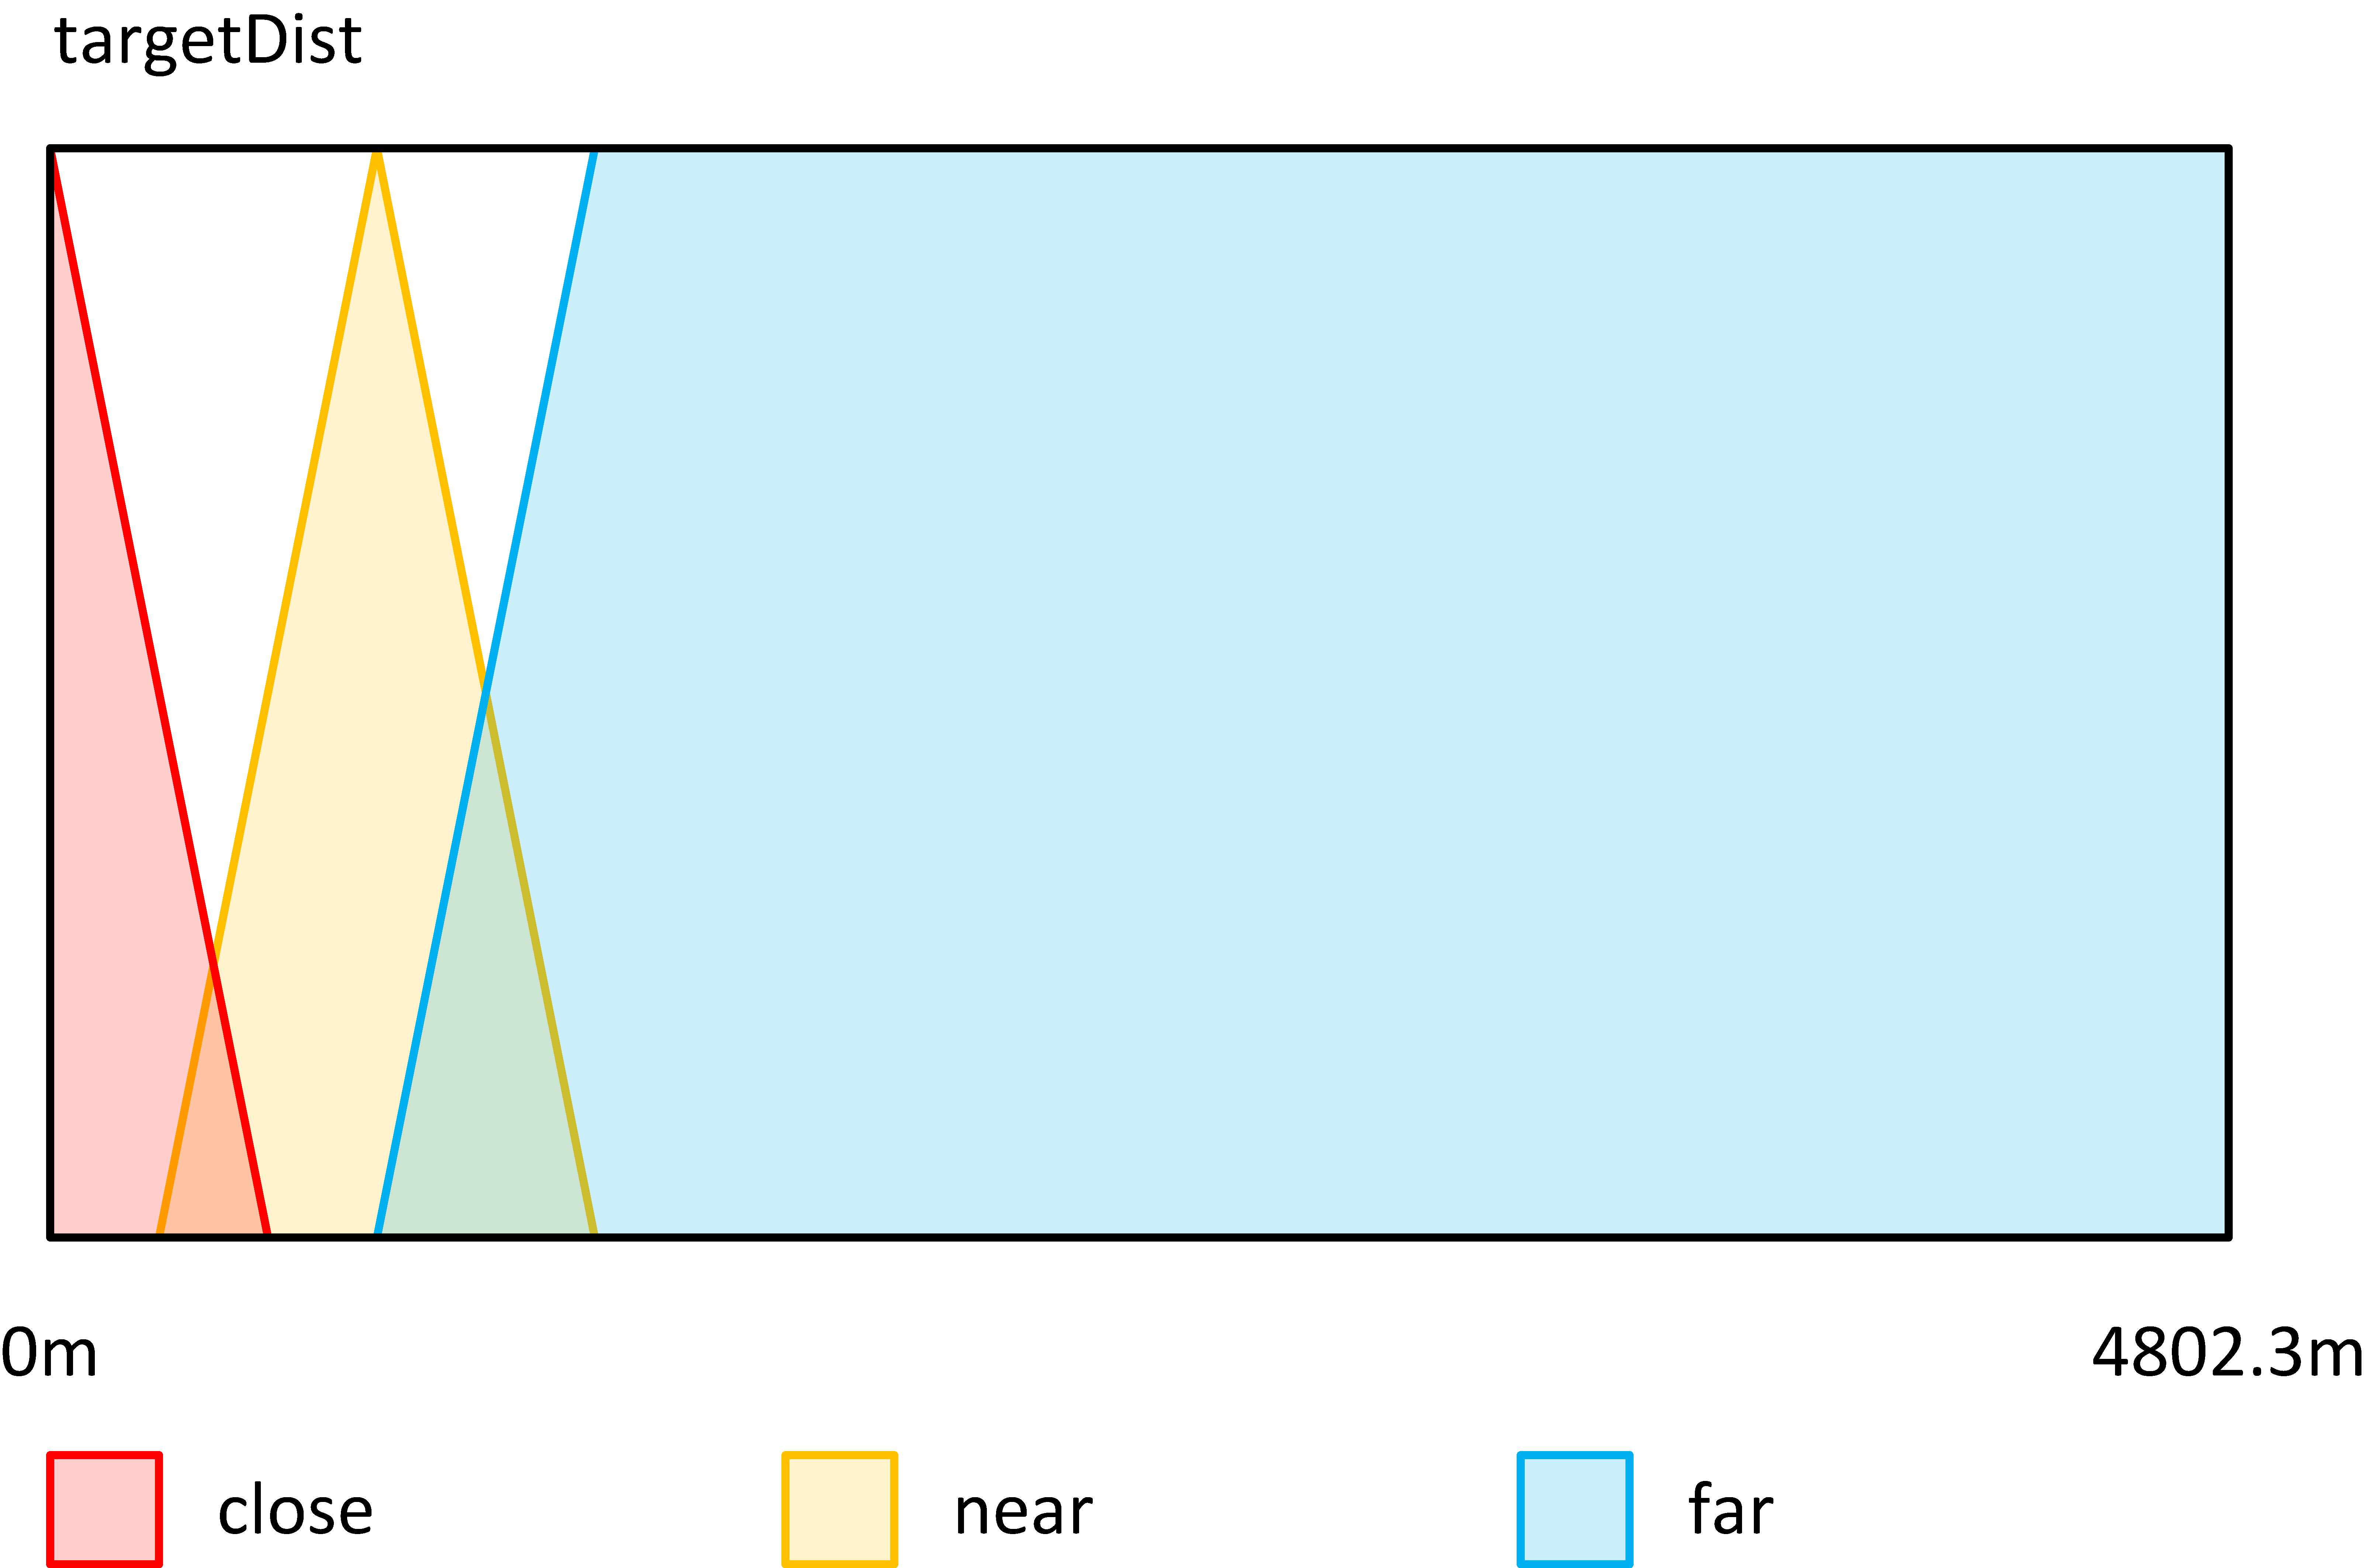
\includegraphics[scale=0.08]{./img/pdf/targetDistSets.pdf}
\end{figure}

\subsubsection{targetAspect}

The linguistic variable \emph{targetAspect} is the direction of the target in relation to the player. The universe of disclosure for \emph{targetAspect} is between -360$^{\circ}$ and +360$^{\circ}$. Positive values rotate to the left, and negative values rotate to the right. The fuzzy sets selected relate to clock positions, similar to what fighter pilots might call out in combat. There are three twelve o'clock positions due to the two revolutions between -360$^{\circ}$ and +360$^{\circ}$.

\begin{figure}[H]
\centering
\caption{\emph{targetAspect} fuzzy sets}
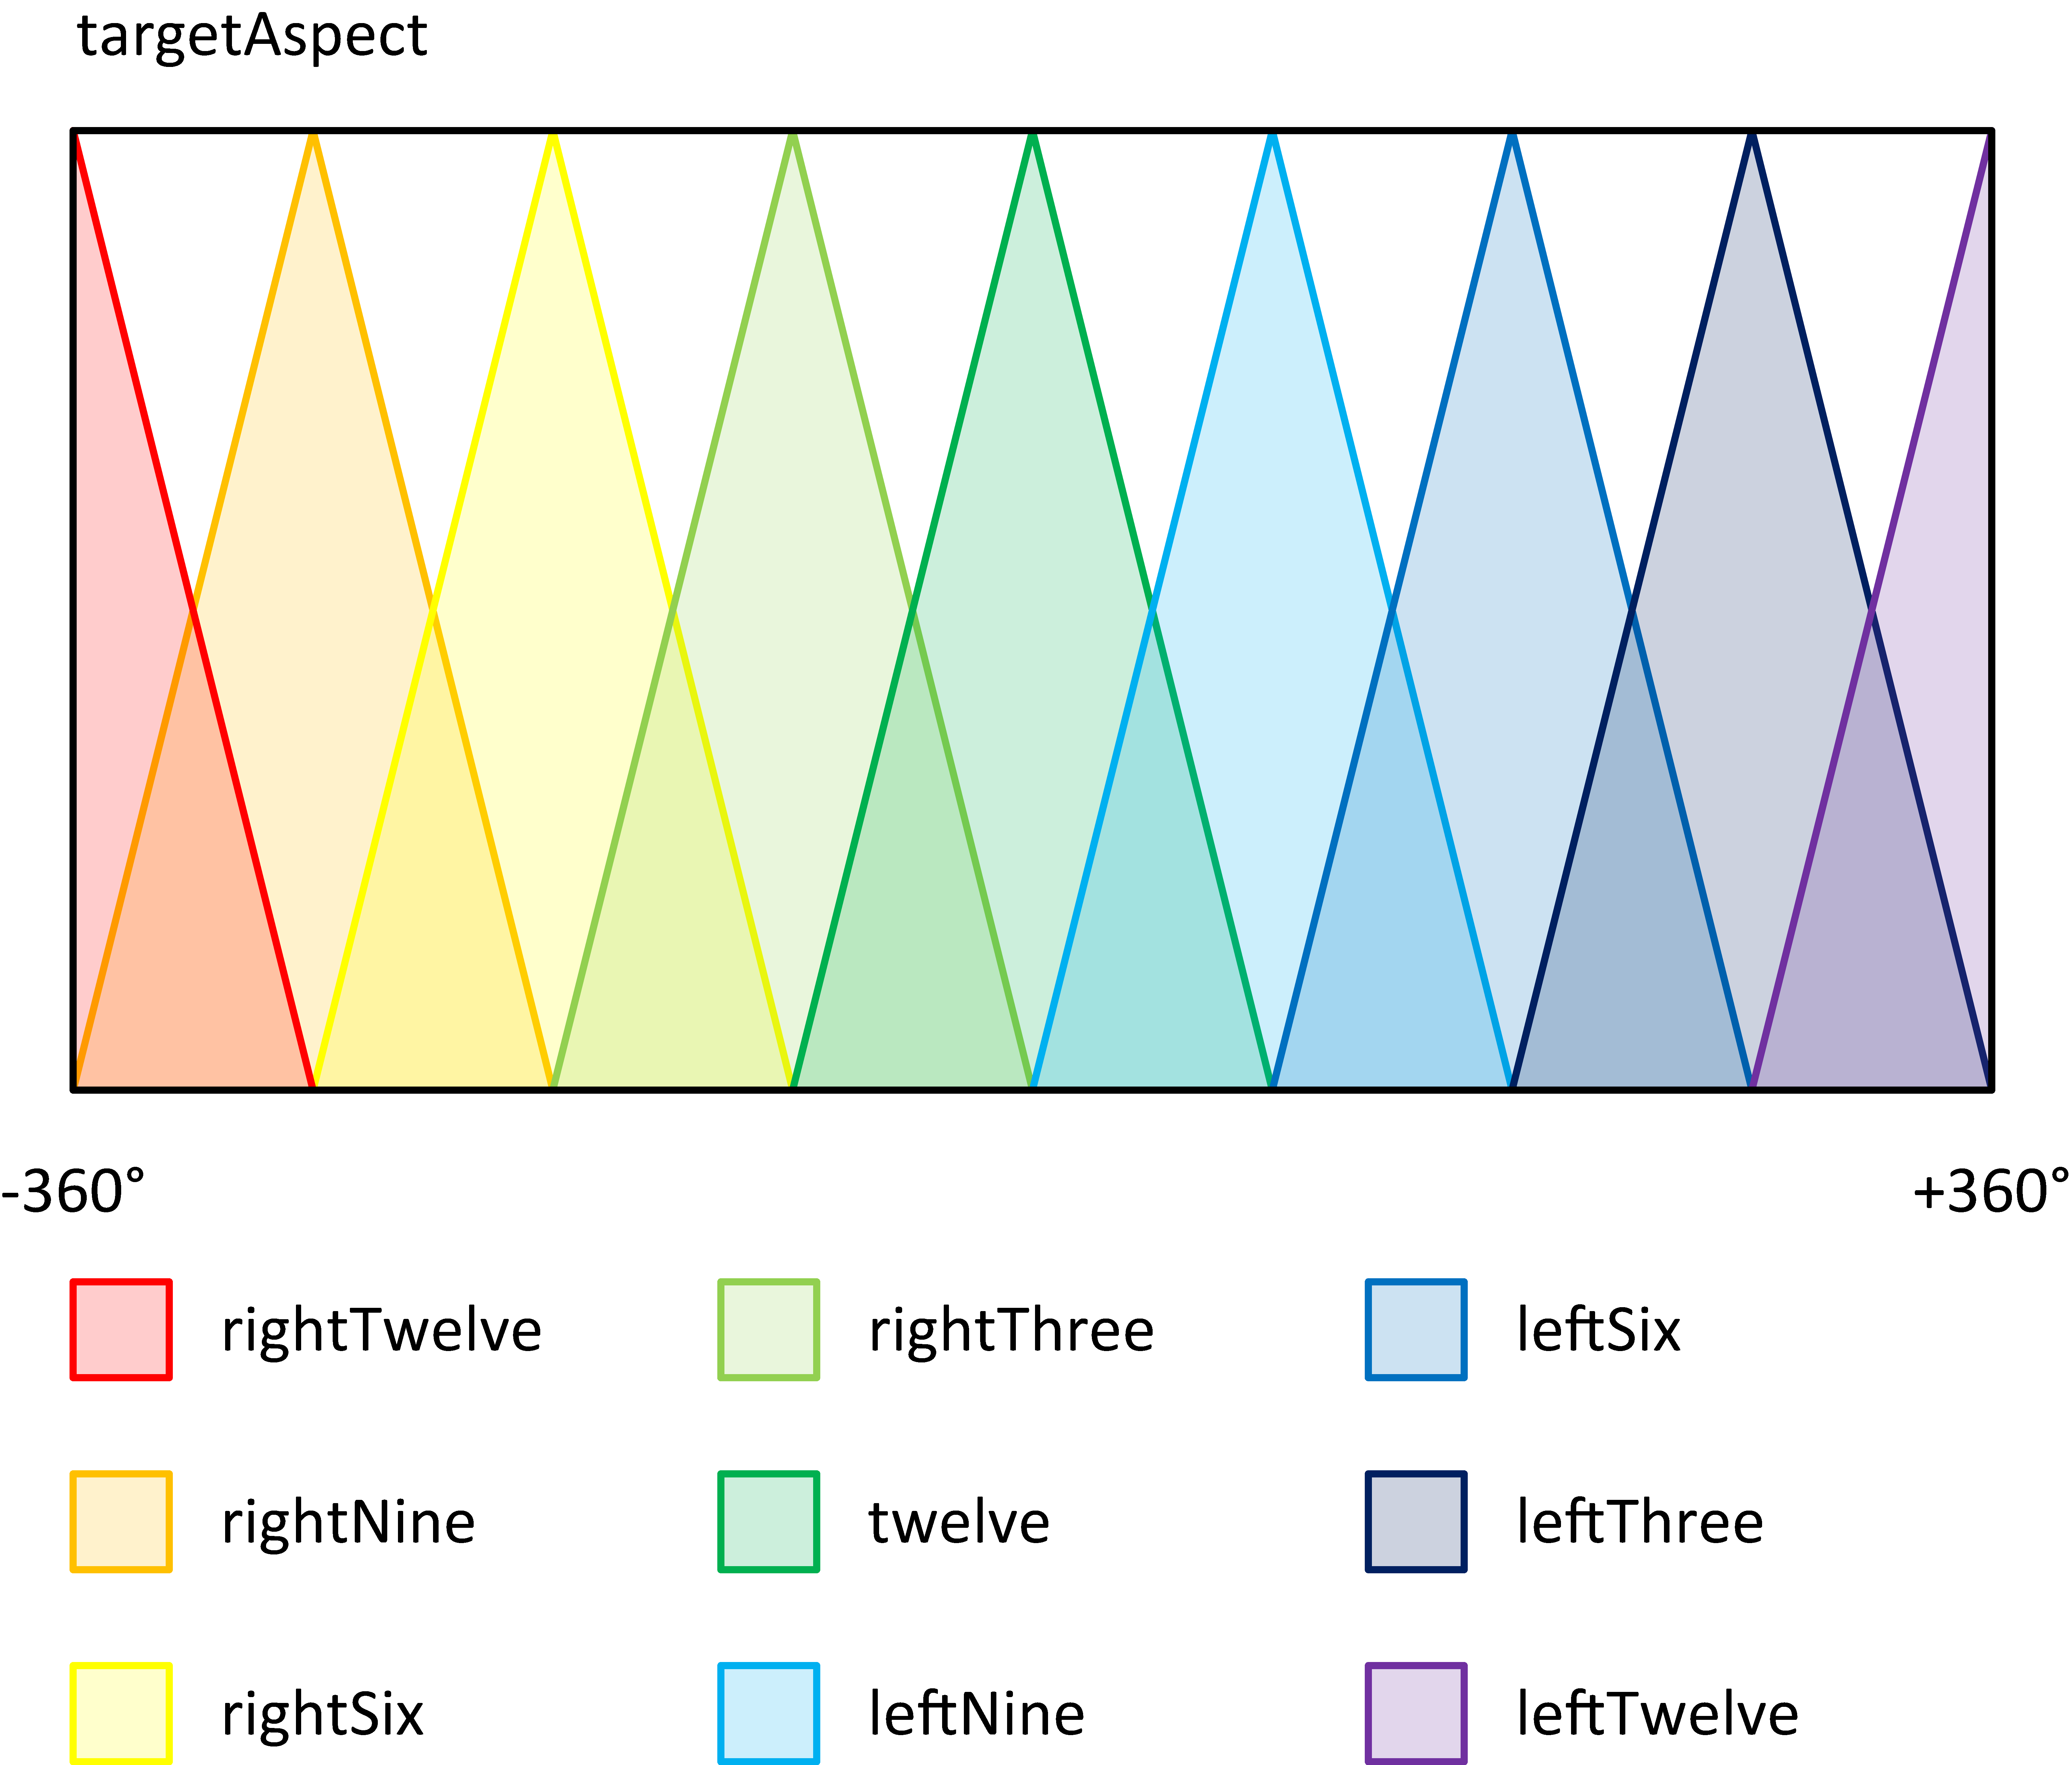
\includegraphics[scale=0.08]{./img/pdf/targetAspectSets.pdf}
\end{figure}

\subsubsection{targetAngleOff}

The linguistic variable \emph{targetAngleOff} relates to the target's current heading, in relation to the player's current heading. For example, if the target is heading towards the player perpendicularly from the right, the target's angle-off would be +90$^{\circ}$. Similarly, if the target has the exact same heading as the player, the target's angle-off would be 0$^{\circ}$. Again, positive values rotate to the left, and negative values rotate to the right. The universe of disclosure is between -360$^{\circ}$ and +360$^{\circ}$. The fuzzy sets selected mimic clock positions, similar to \emph{targetAspect}, however are named with degree values. A merge is when the player and target have opposite angle-off's, ie. 180$^{\circ}$. In this situation, if the player and target were in front of each other, they would facing each other, and would be about to directly pass each other, in a ``merge''.

\begin{figure}[H]
\centering
\caption{\emph{targetAngleOff} fuzzy sets}
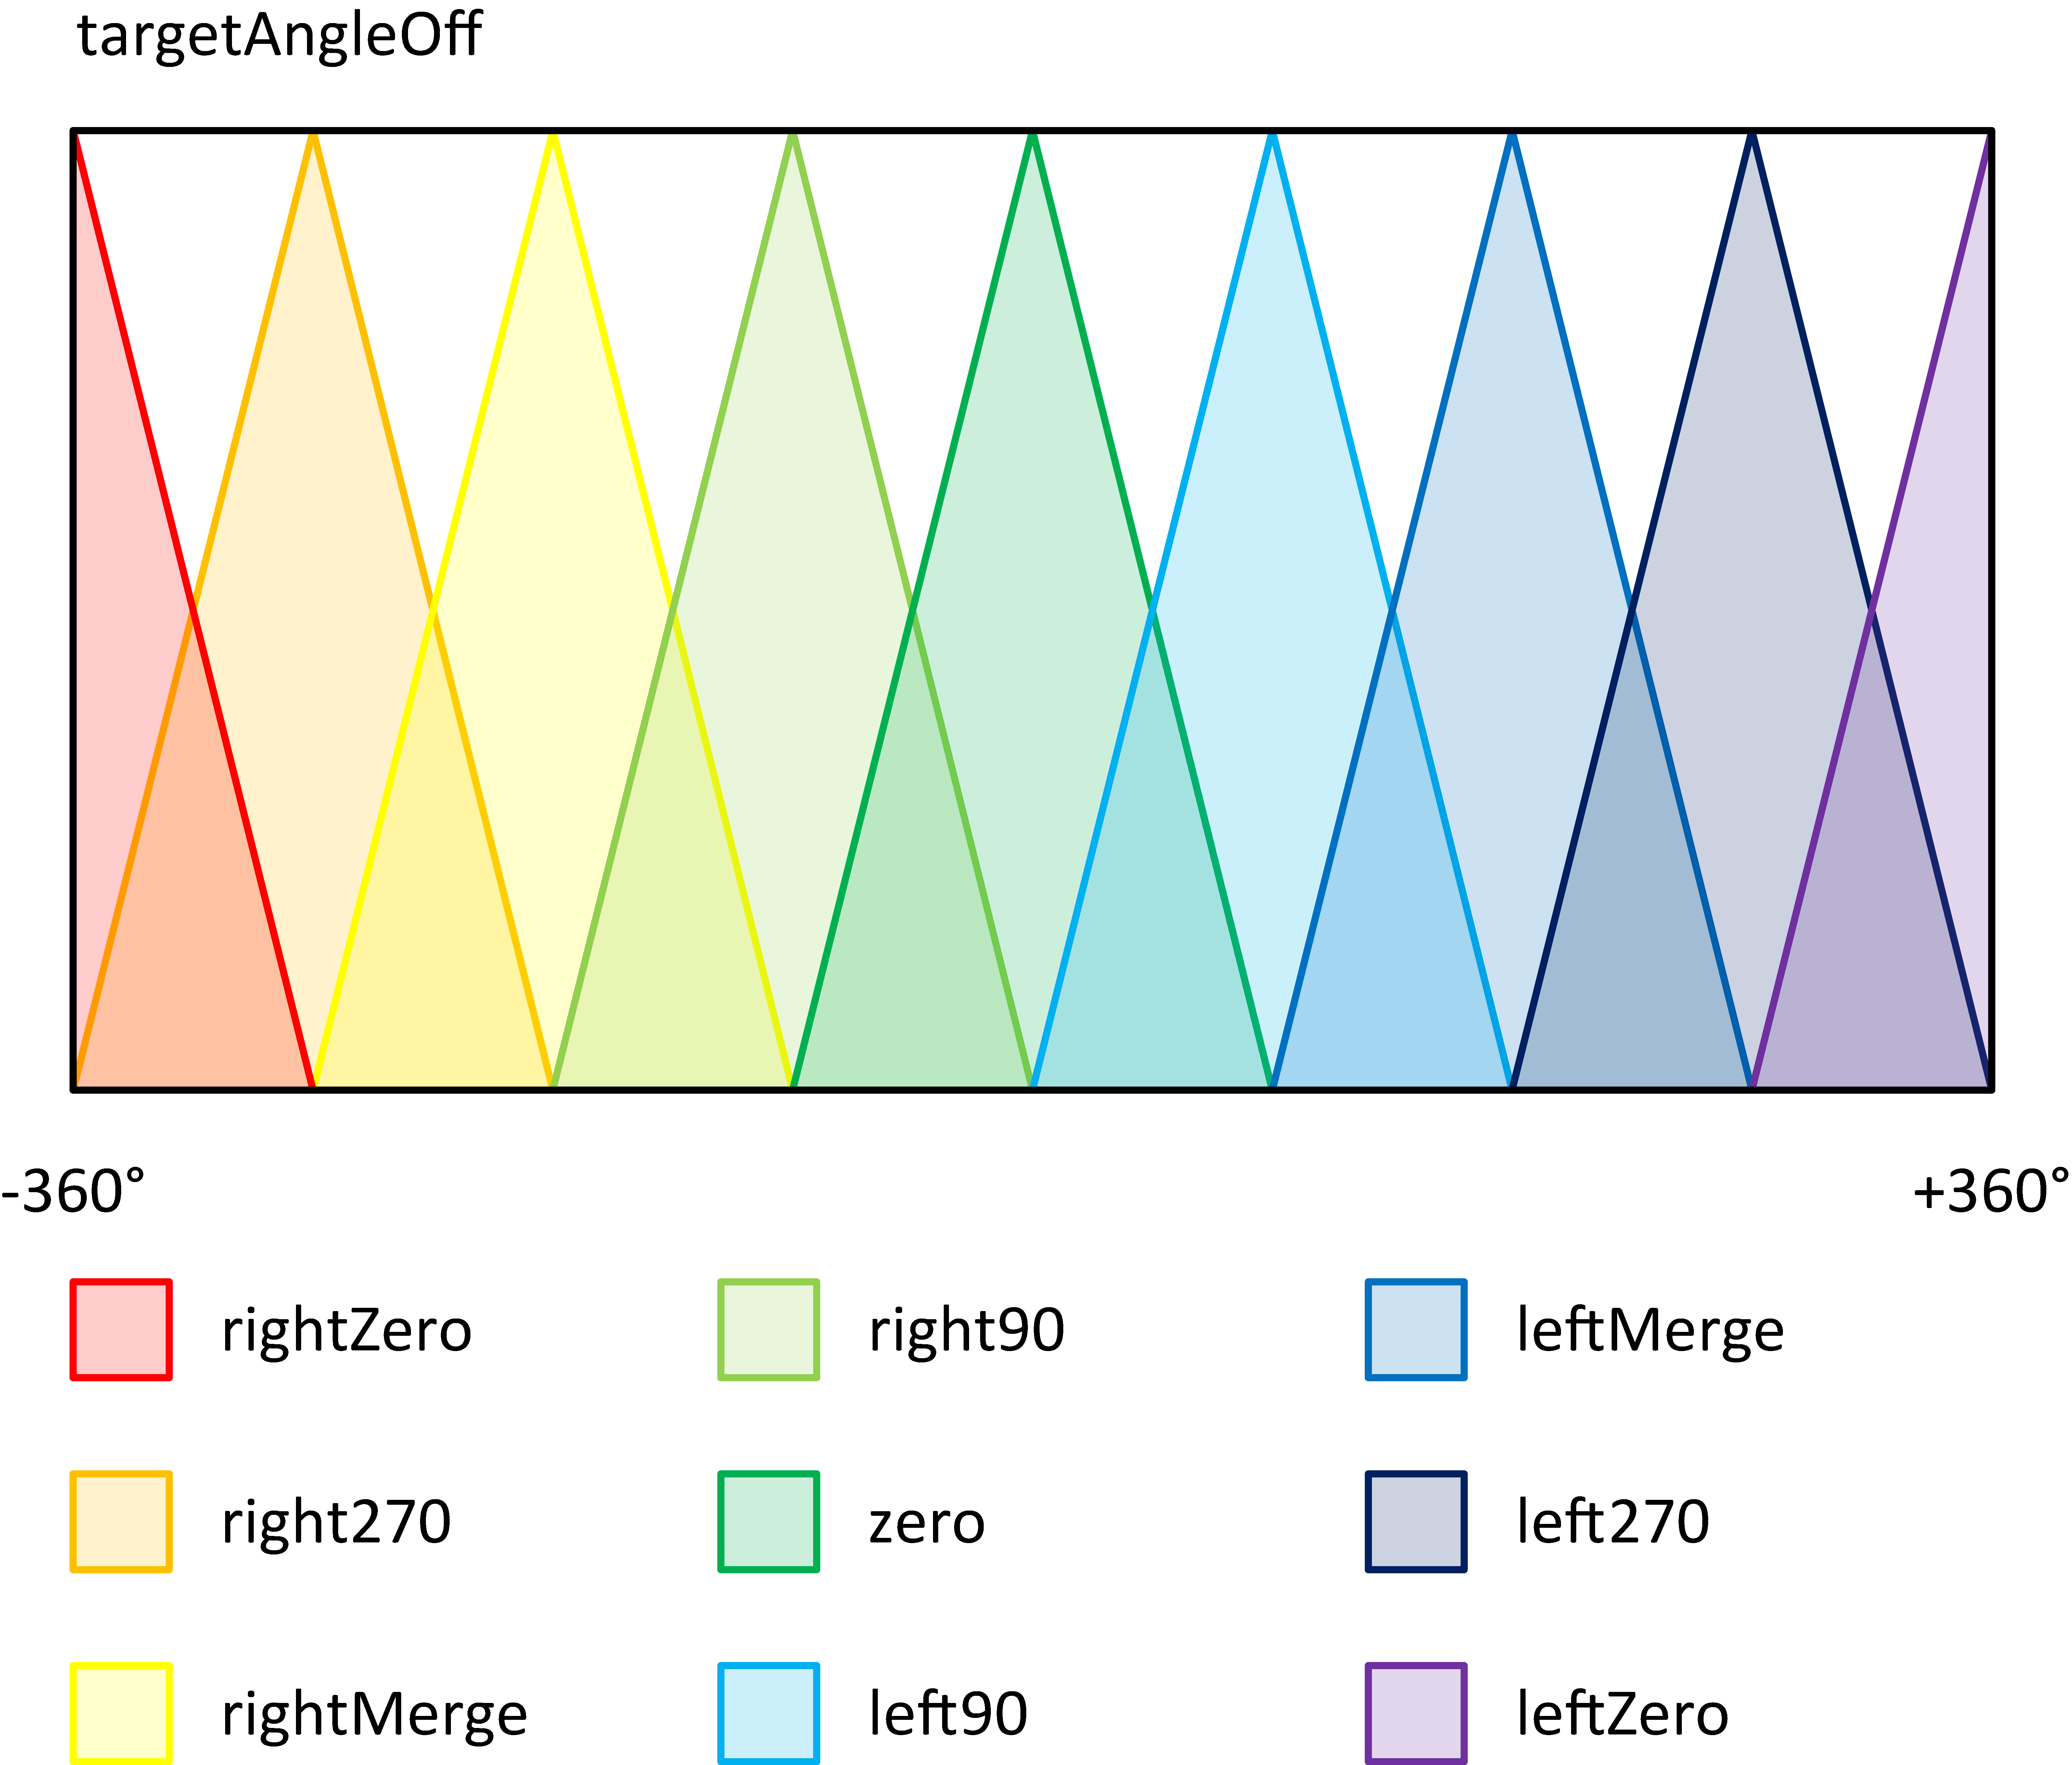
\includegraphics[scale=0.08]{./img/pdf/targetAngleOffSets.pdf}
\end{figure}

\subsubsection{targetEnergyDiff}

The linguistic variable \emph{targetEnergyDiff} relates to the difference between the player's energy and the current target's energy. The universe of disclosure for \emph{targetEnergyDiff} is between -10,000j and +10,000j. The fuzzy sets selected for this linguistic variable are \emph{losing} and \emph{winning}.

\begin{figure}[H]
\centering
\caption{\emph{targetEnergyDiff} fuzzy sets}
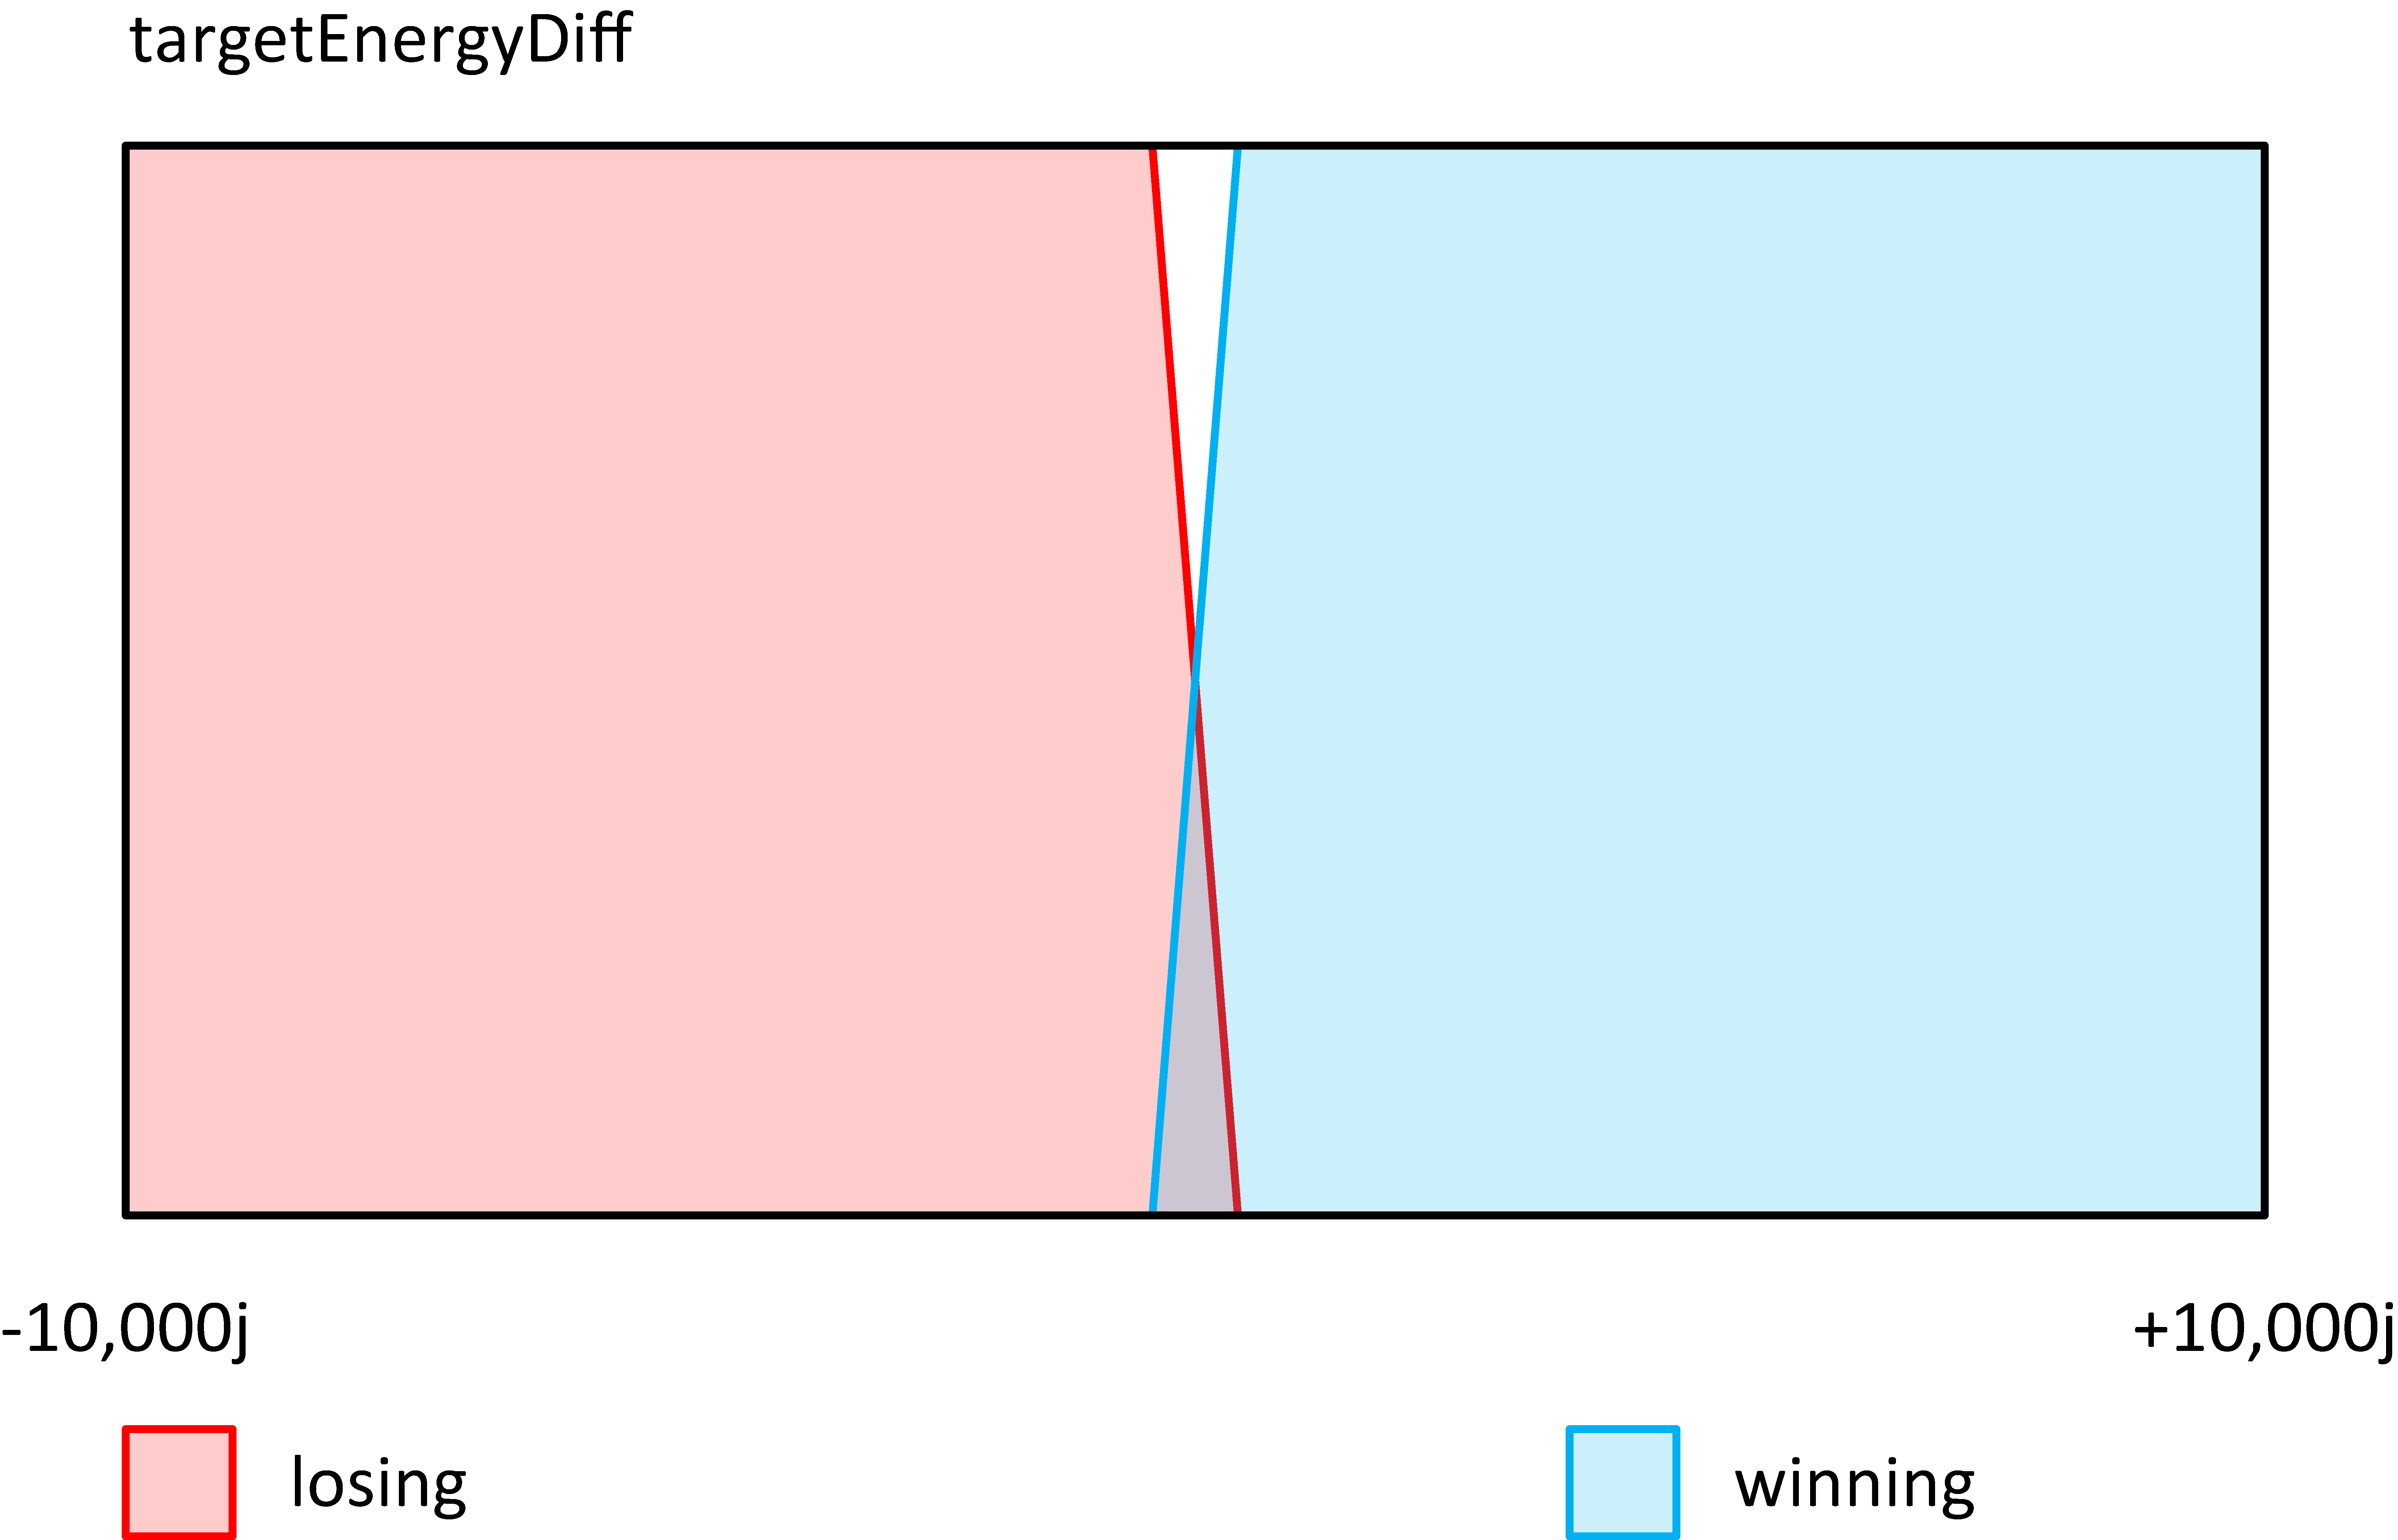
\includegraphics[scale=0.08]{./img/pdf/targetEnergyDiffSets.pdf}
\end{figure}

\subsection{Blast variables}

The sensor returns a list of all energy blasts currently in the battle space. This controller only considers the closest energy blast to dodge, and ignores all other blasts in the list.

\subsubsection{blastDist}

The linguistic variable \emph{blastDist} is the distance from the player to the energy blast. The universe of disclosure for \emph{blastDist} is between 0m and 4802.3m, and the fuzzy sets are defined as \emph{close} and \emph{far}.

\begin{figure}[H]
\centering
\caption{\emph{blastDist} fuzzy sets}
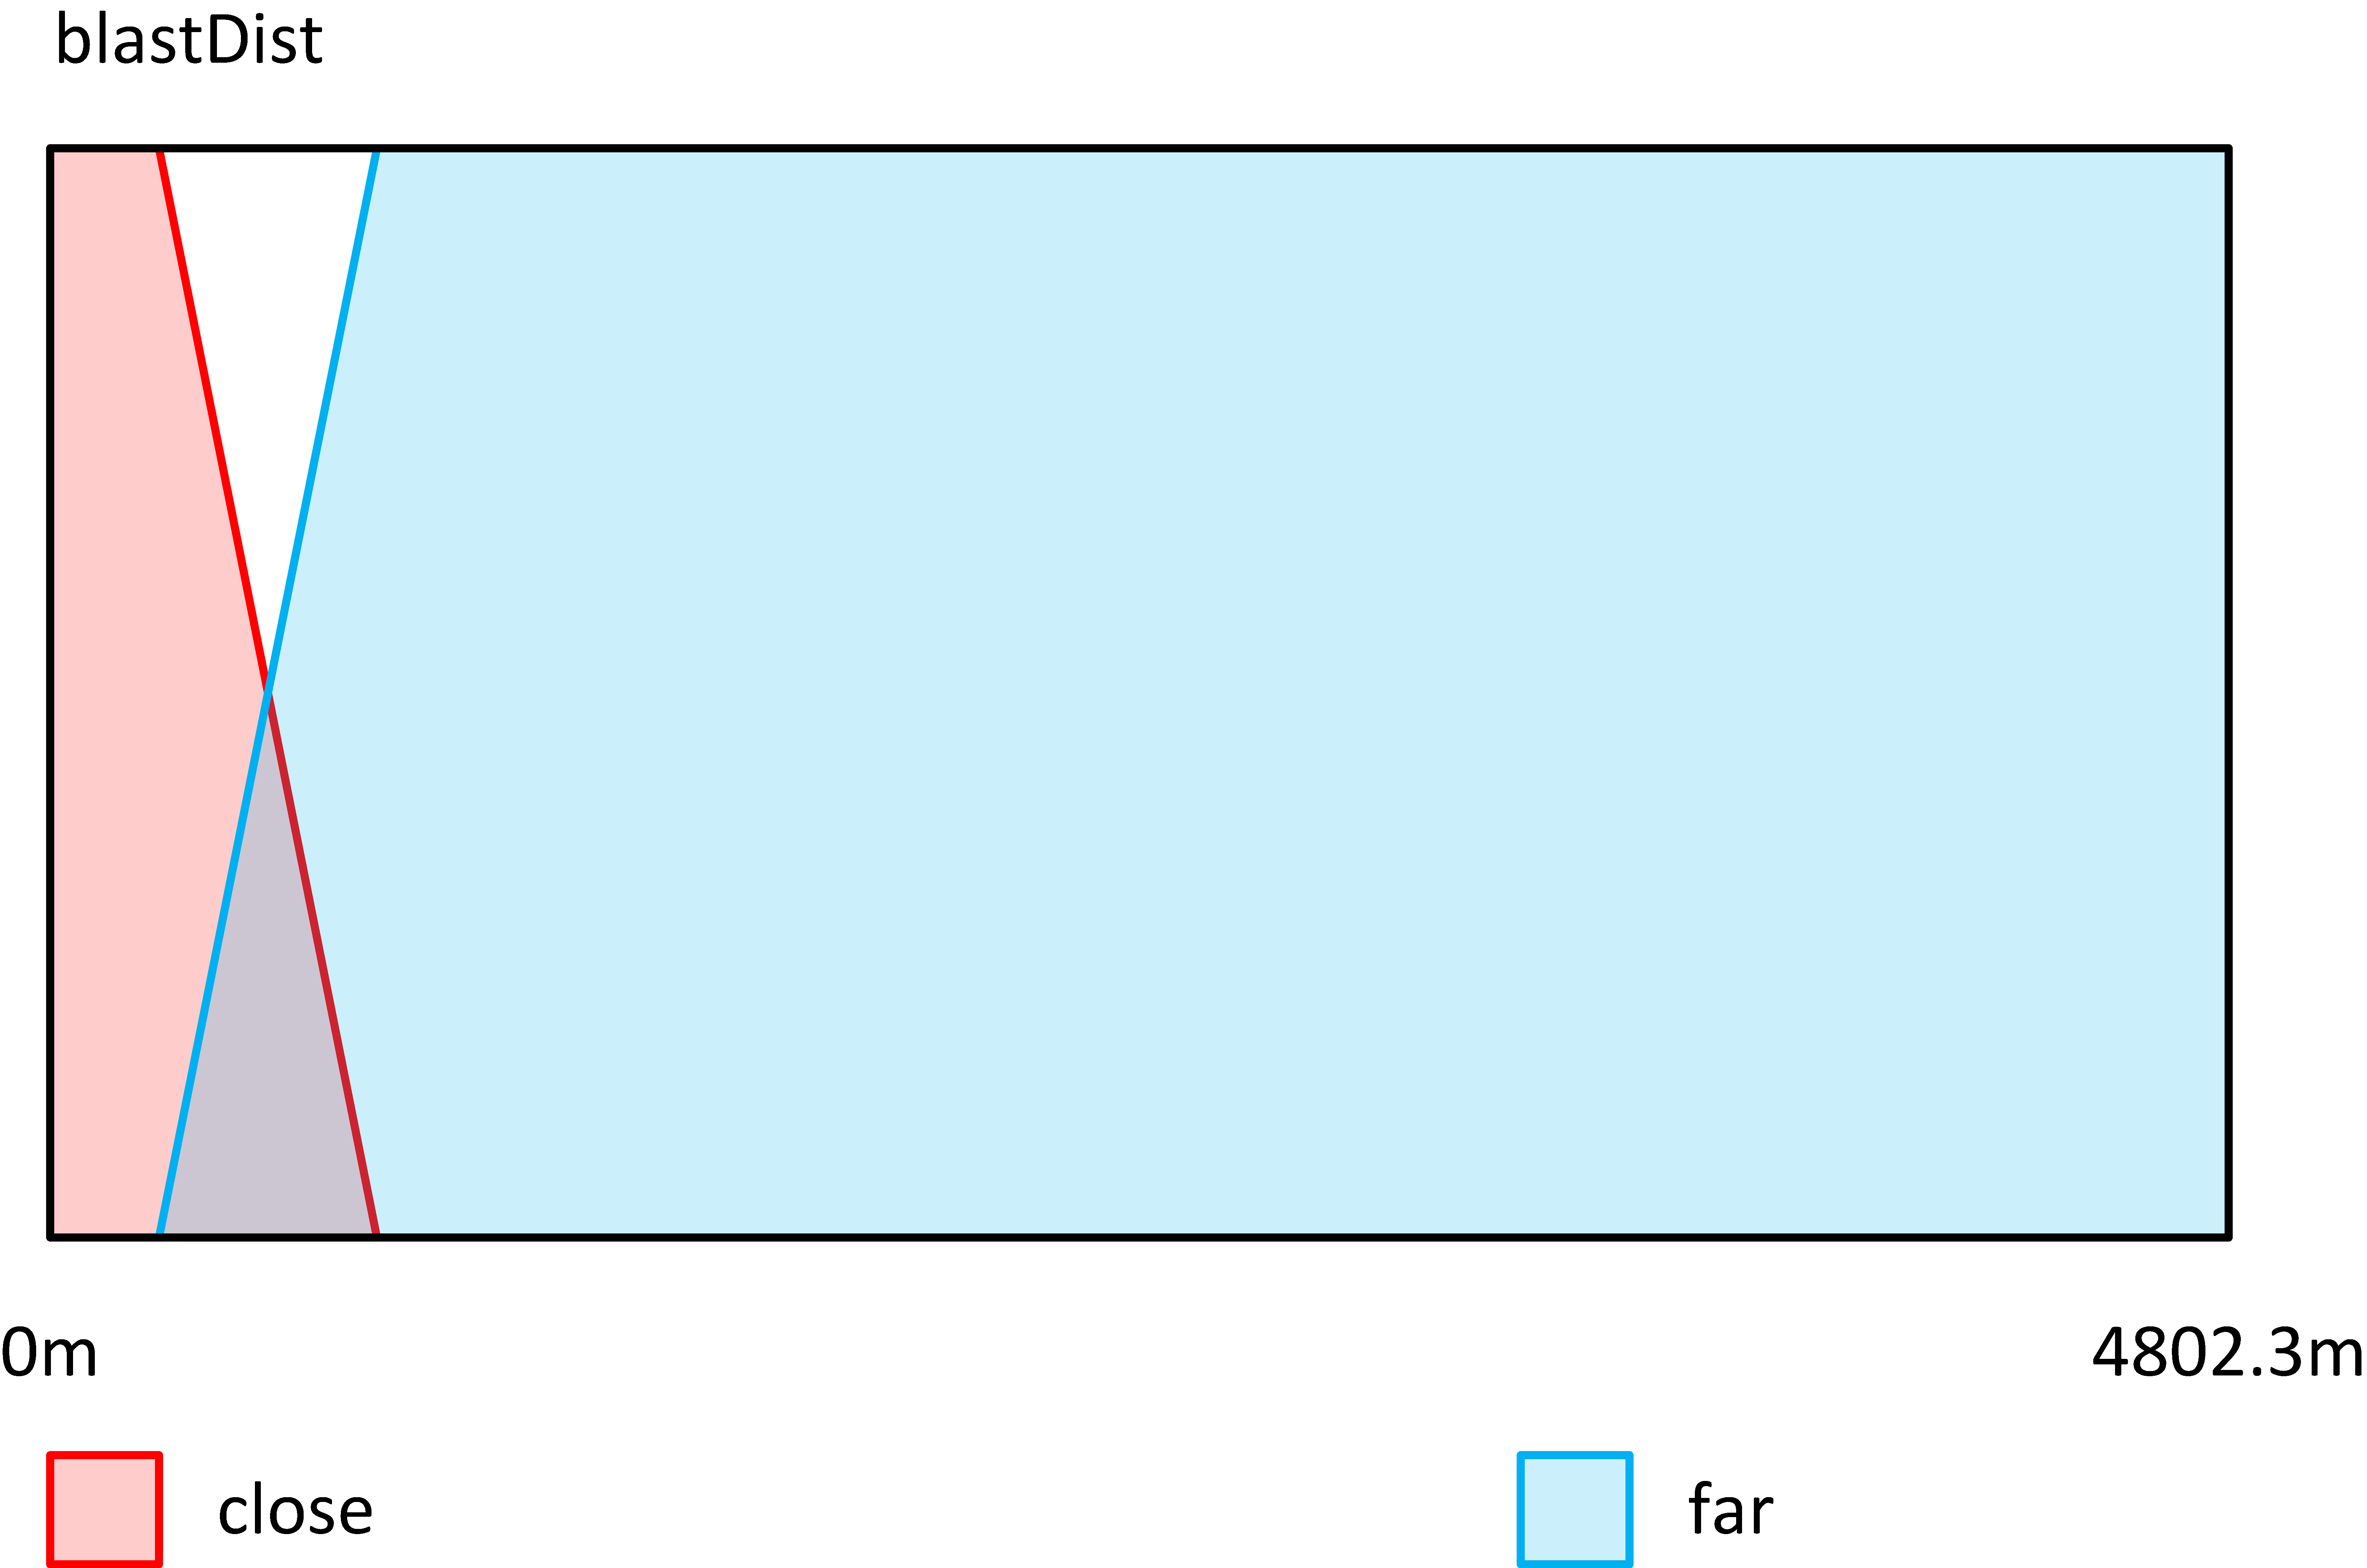
\includegraphics[scale=0.08]{./img/pdf/blastDistSets.pdf}
\end{figure}

\subsubsection{blastAspect}

The linguistic variable \emph{blastAspect} is similar to \emph{targetAspect}, but relates to the direction from the player to the energy blast. Similar fuzzy sets, based on the clock analogy have been used.

\begin{figure}[H]
\centering
\caption{\emph{blastAspect} fuzzy sets}
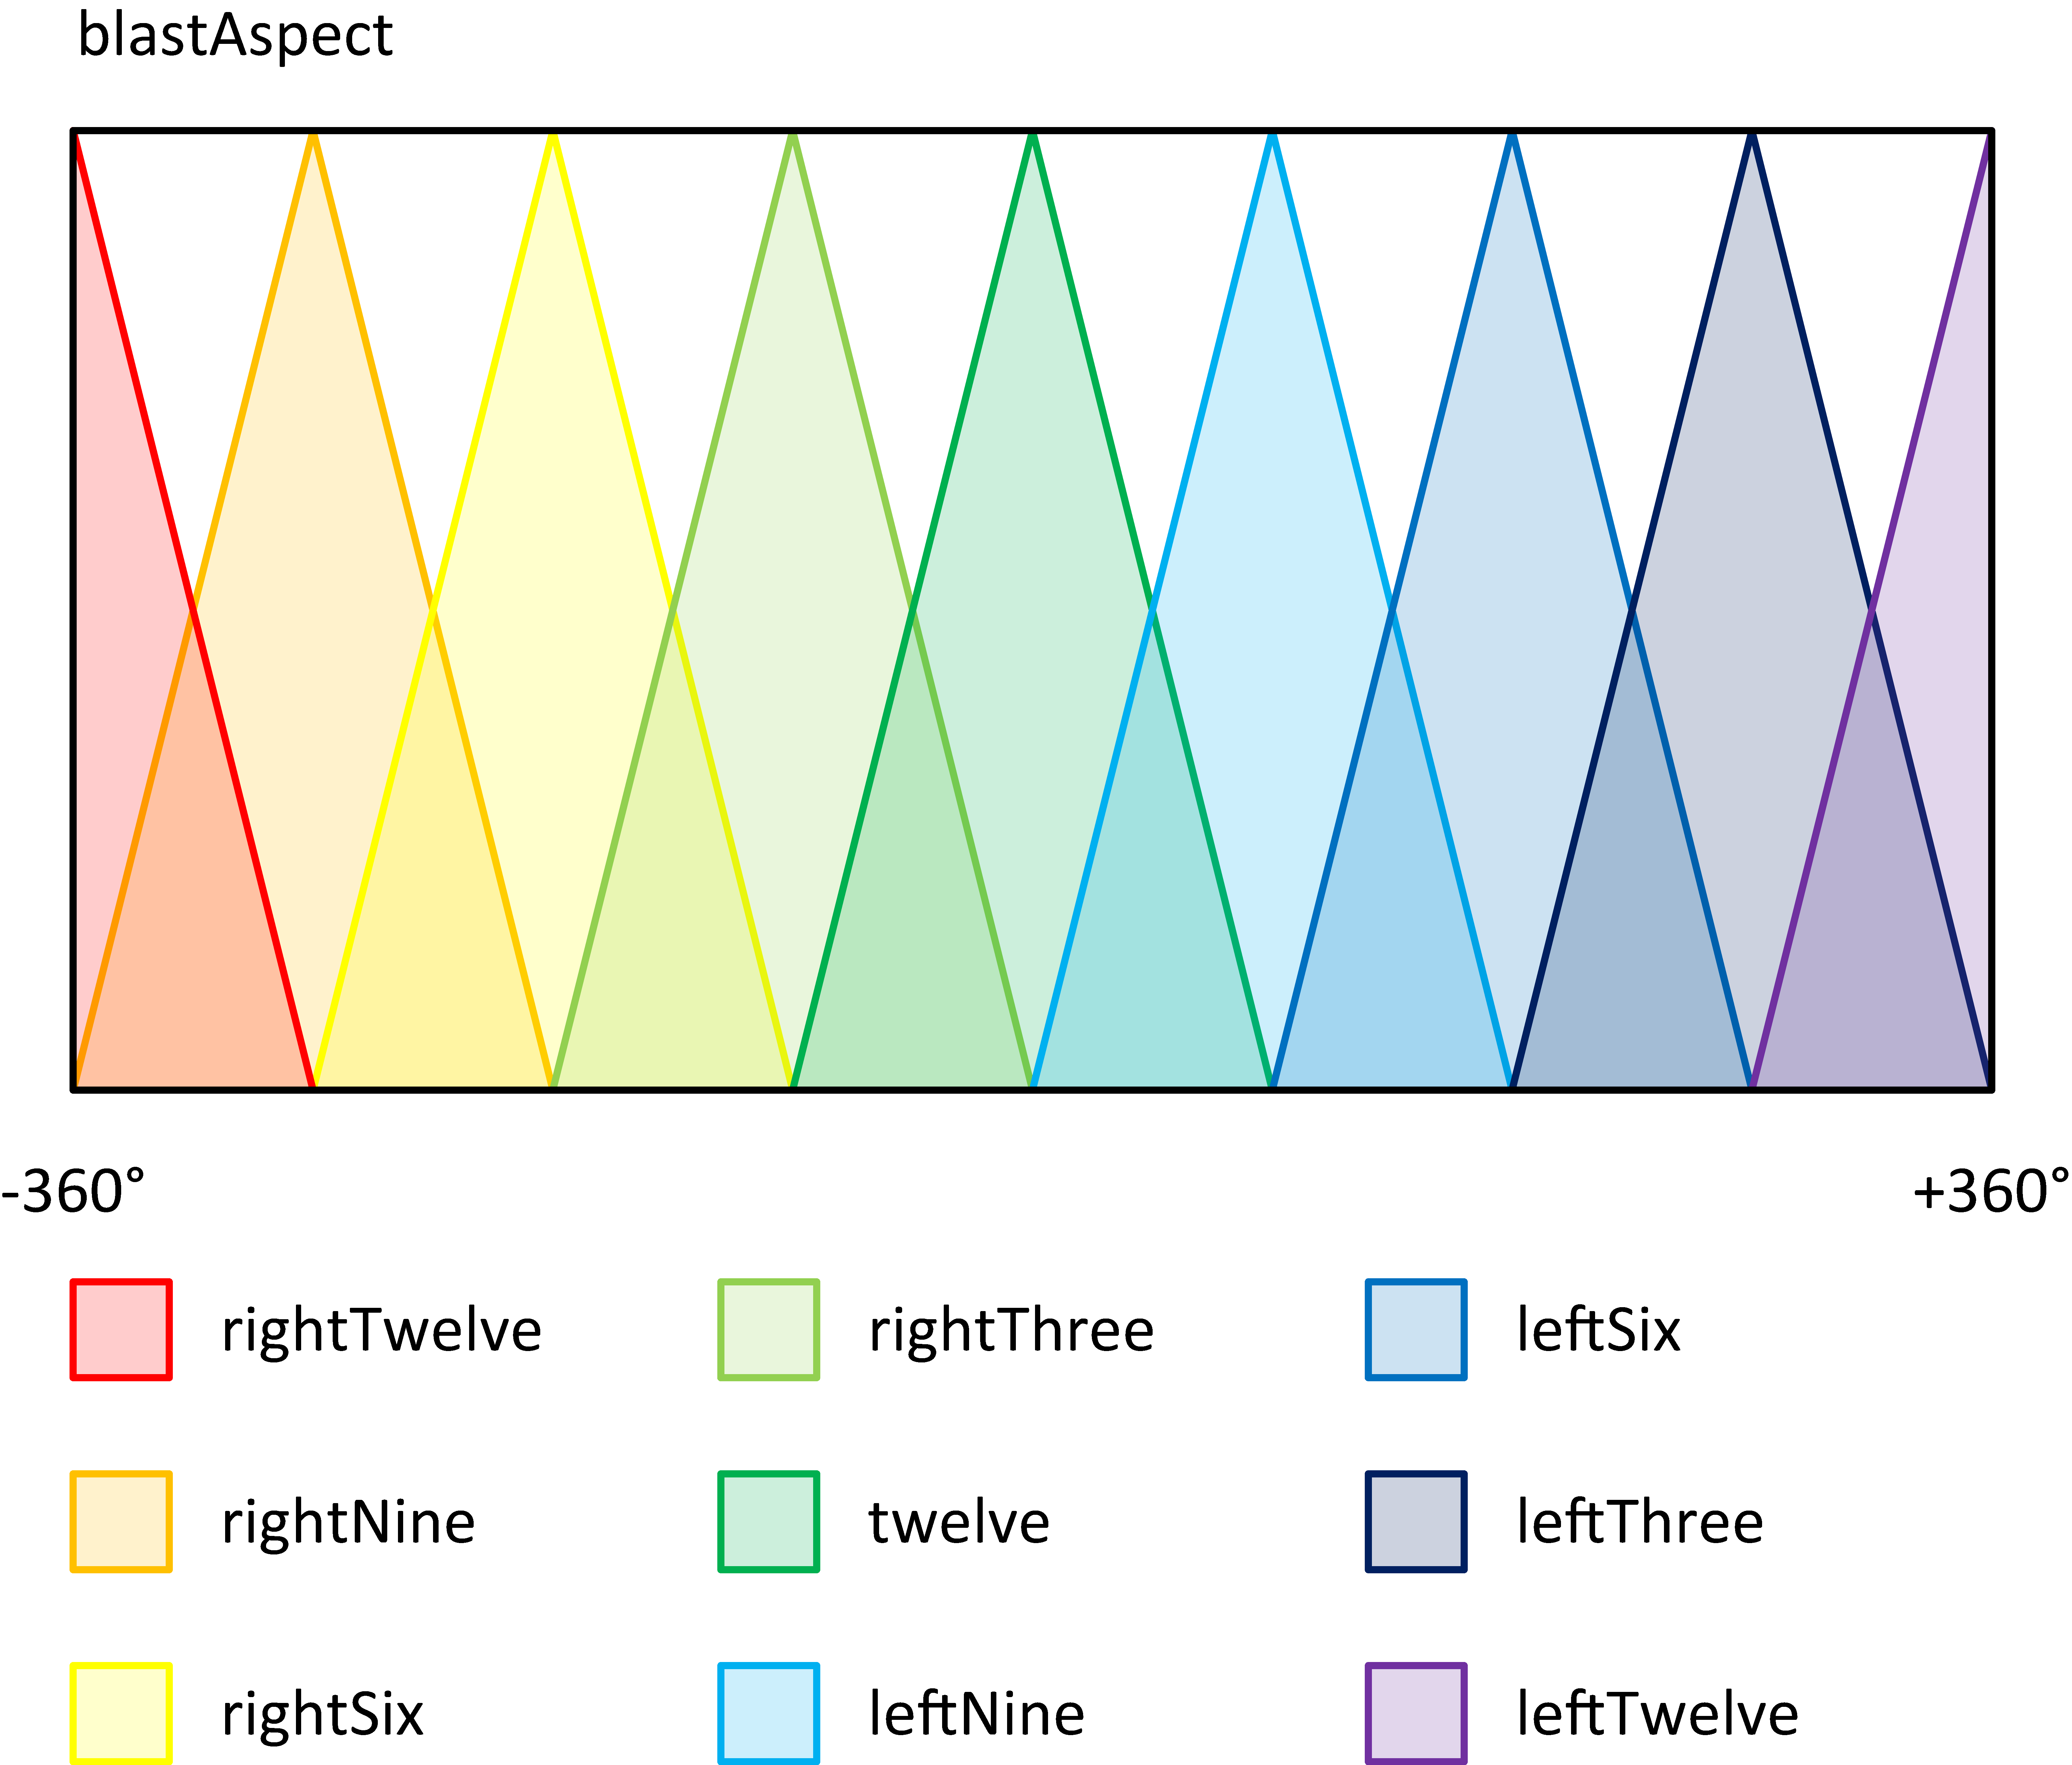
\includegraphics[scale=0.08]{./img/pdf/blastAspectSets.pdf}
\end{figure}

\subsubsection{blastAngleOff}

The linguistic variable \emph{blastAngleOff} is similar to \emph{targetAngleOff}, but references the current heading of the energy blast in relation to the player's heading. Similar fuzzy sets have also been used.

\begin{figure}[H]
\centering
\caption{\emph{blastAngleOff} fuzzy sets}
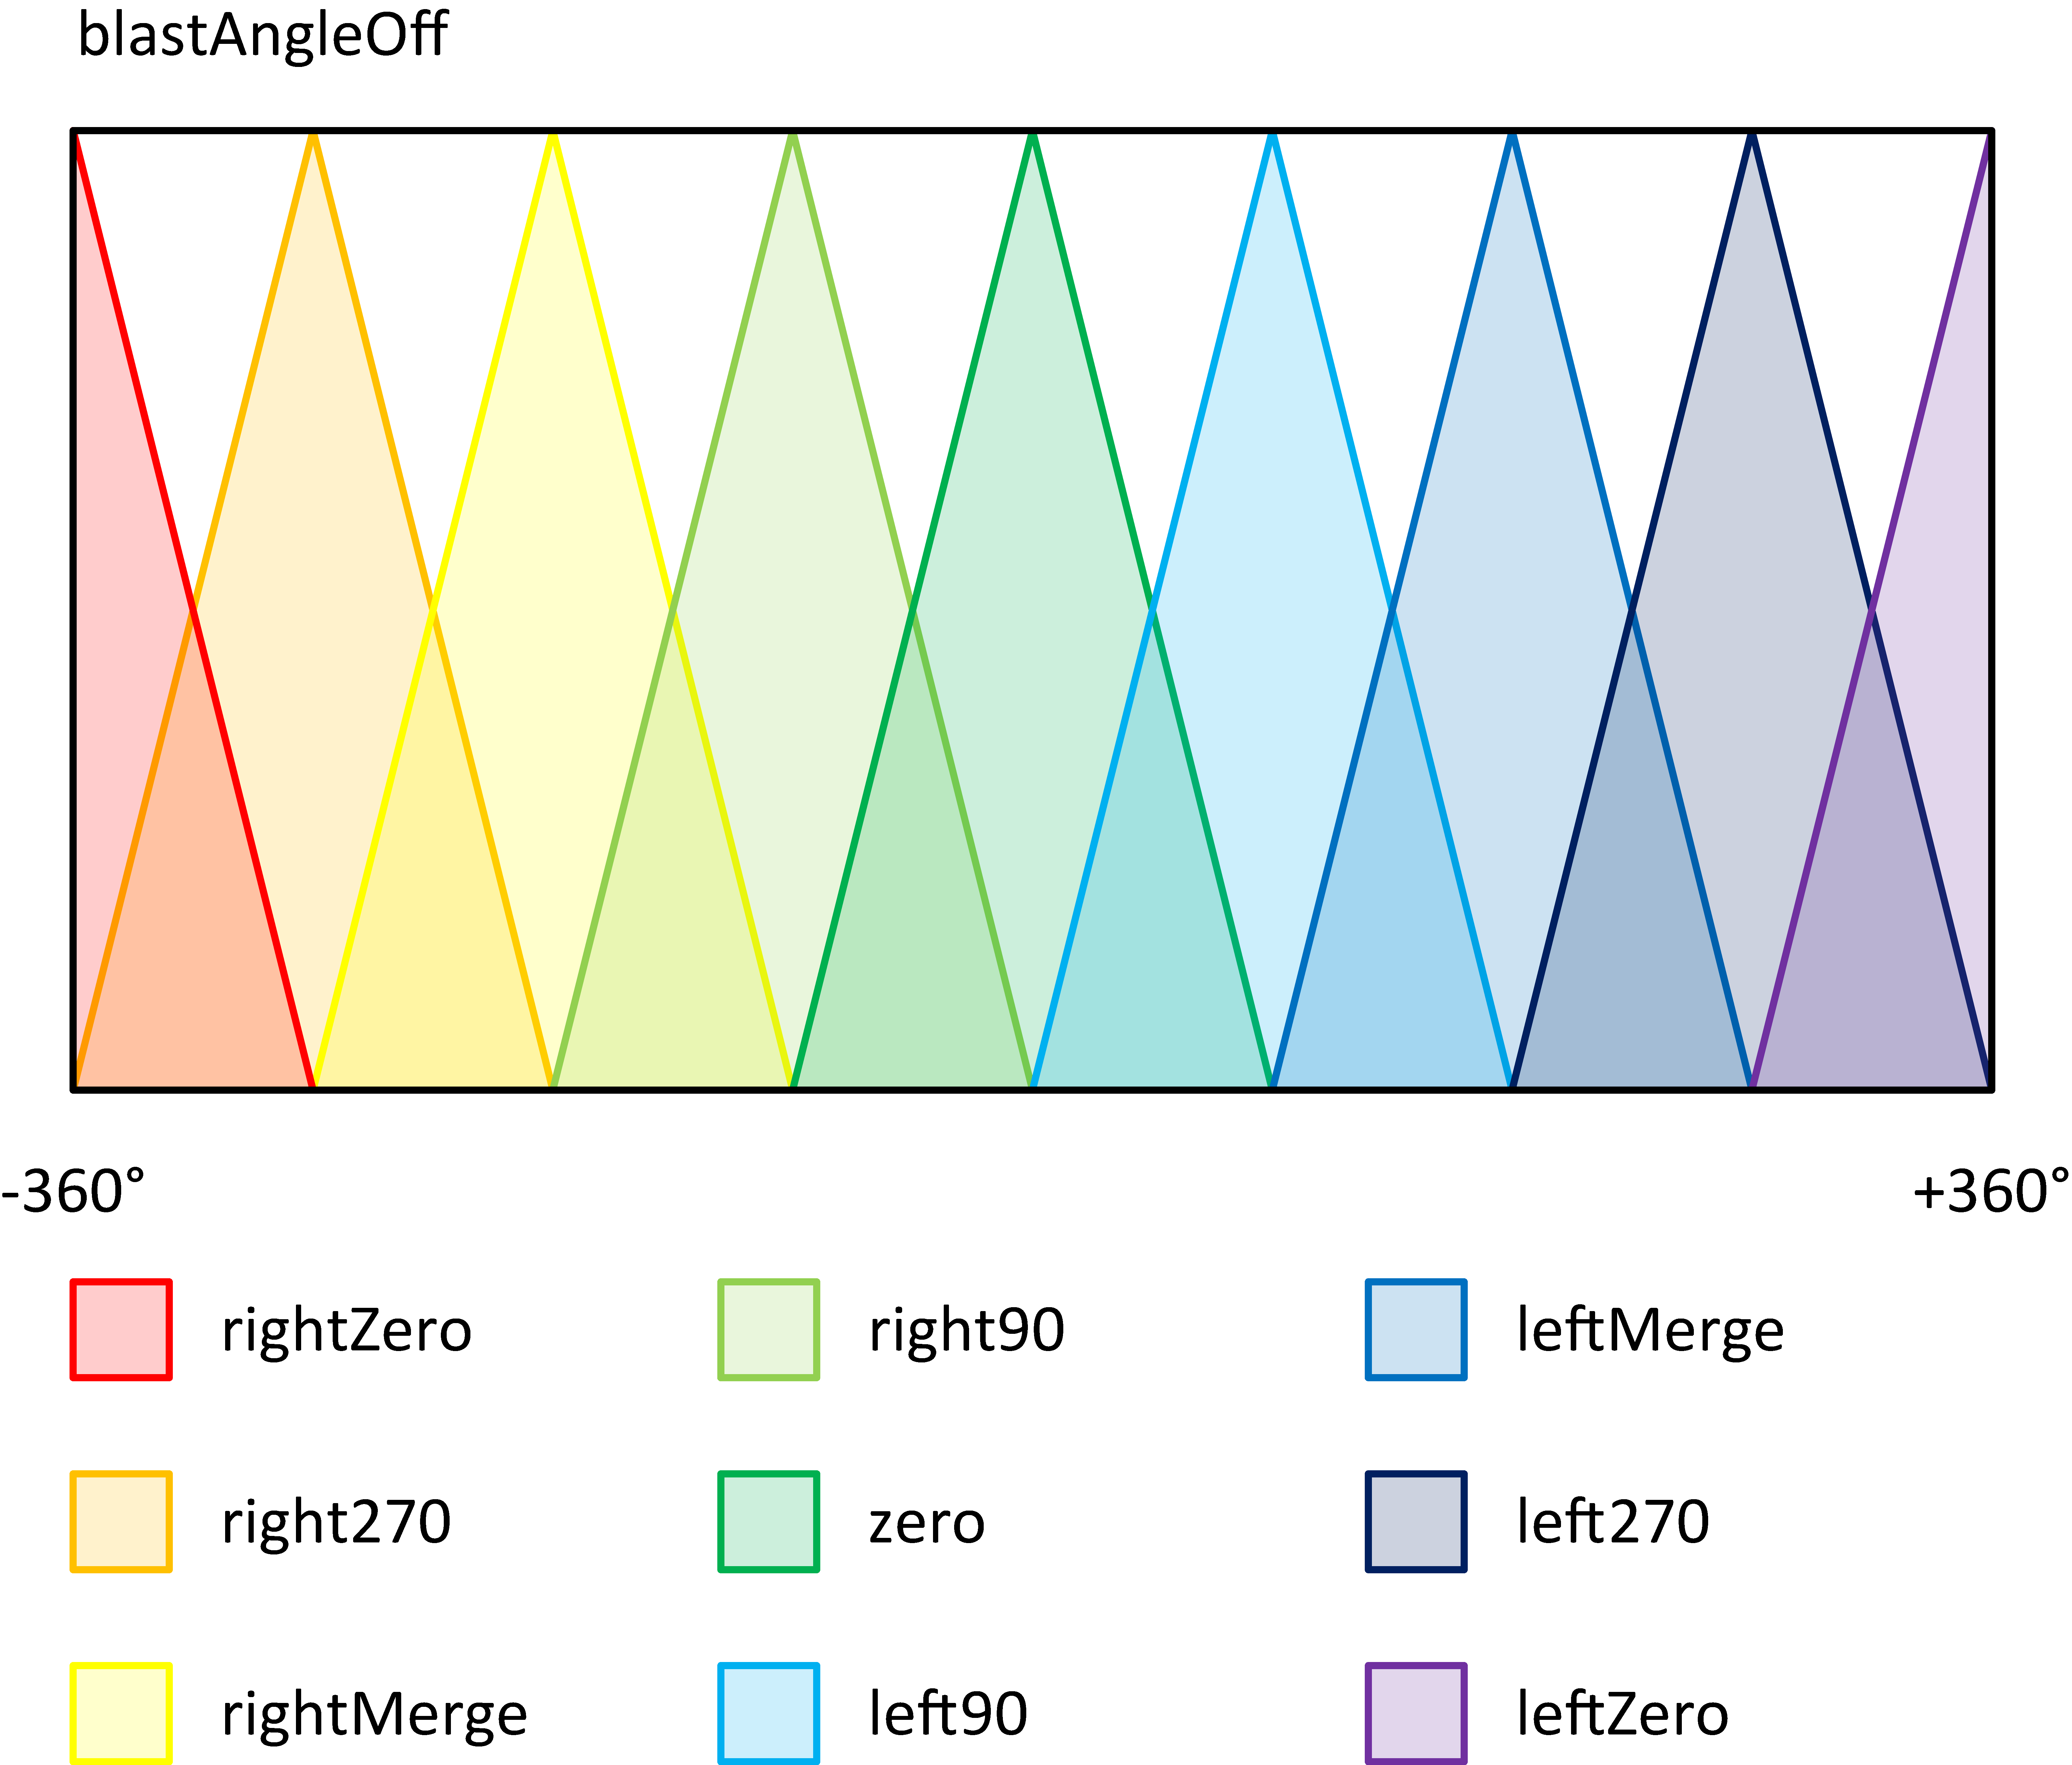
\includegraphics[scale=0.08]{./img/pdf/blastAngleOffSets.pdf}
\end{figure}

\subsection{Powerup variables}

The sensor returns a list of all powerups that currently exist in the battle space. To conserve energy, this controller only reacts to powerups only if they are nearby, and assumes that powerups that are far would most likely be consumed by an enemy by the time the player arrives.

\subsubsection{powerUpDist}

The linguistic variable \emph{powerUpDist} is the distance between the target and the powerup. Similar to \emph{targetDist}, the universe of disclosure is between 0m and 4802.3m. Similar fuzzy sets have also been used.

\begin{figure}[H]
\centering
\caption{\emph{powerUpDist} fuzzy sets}
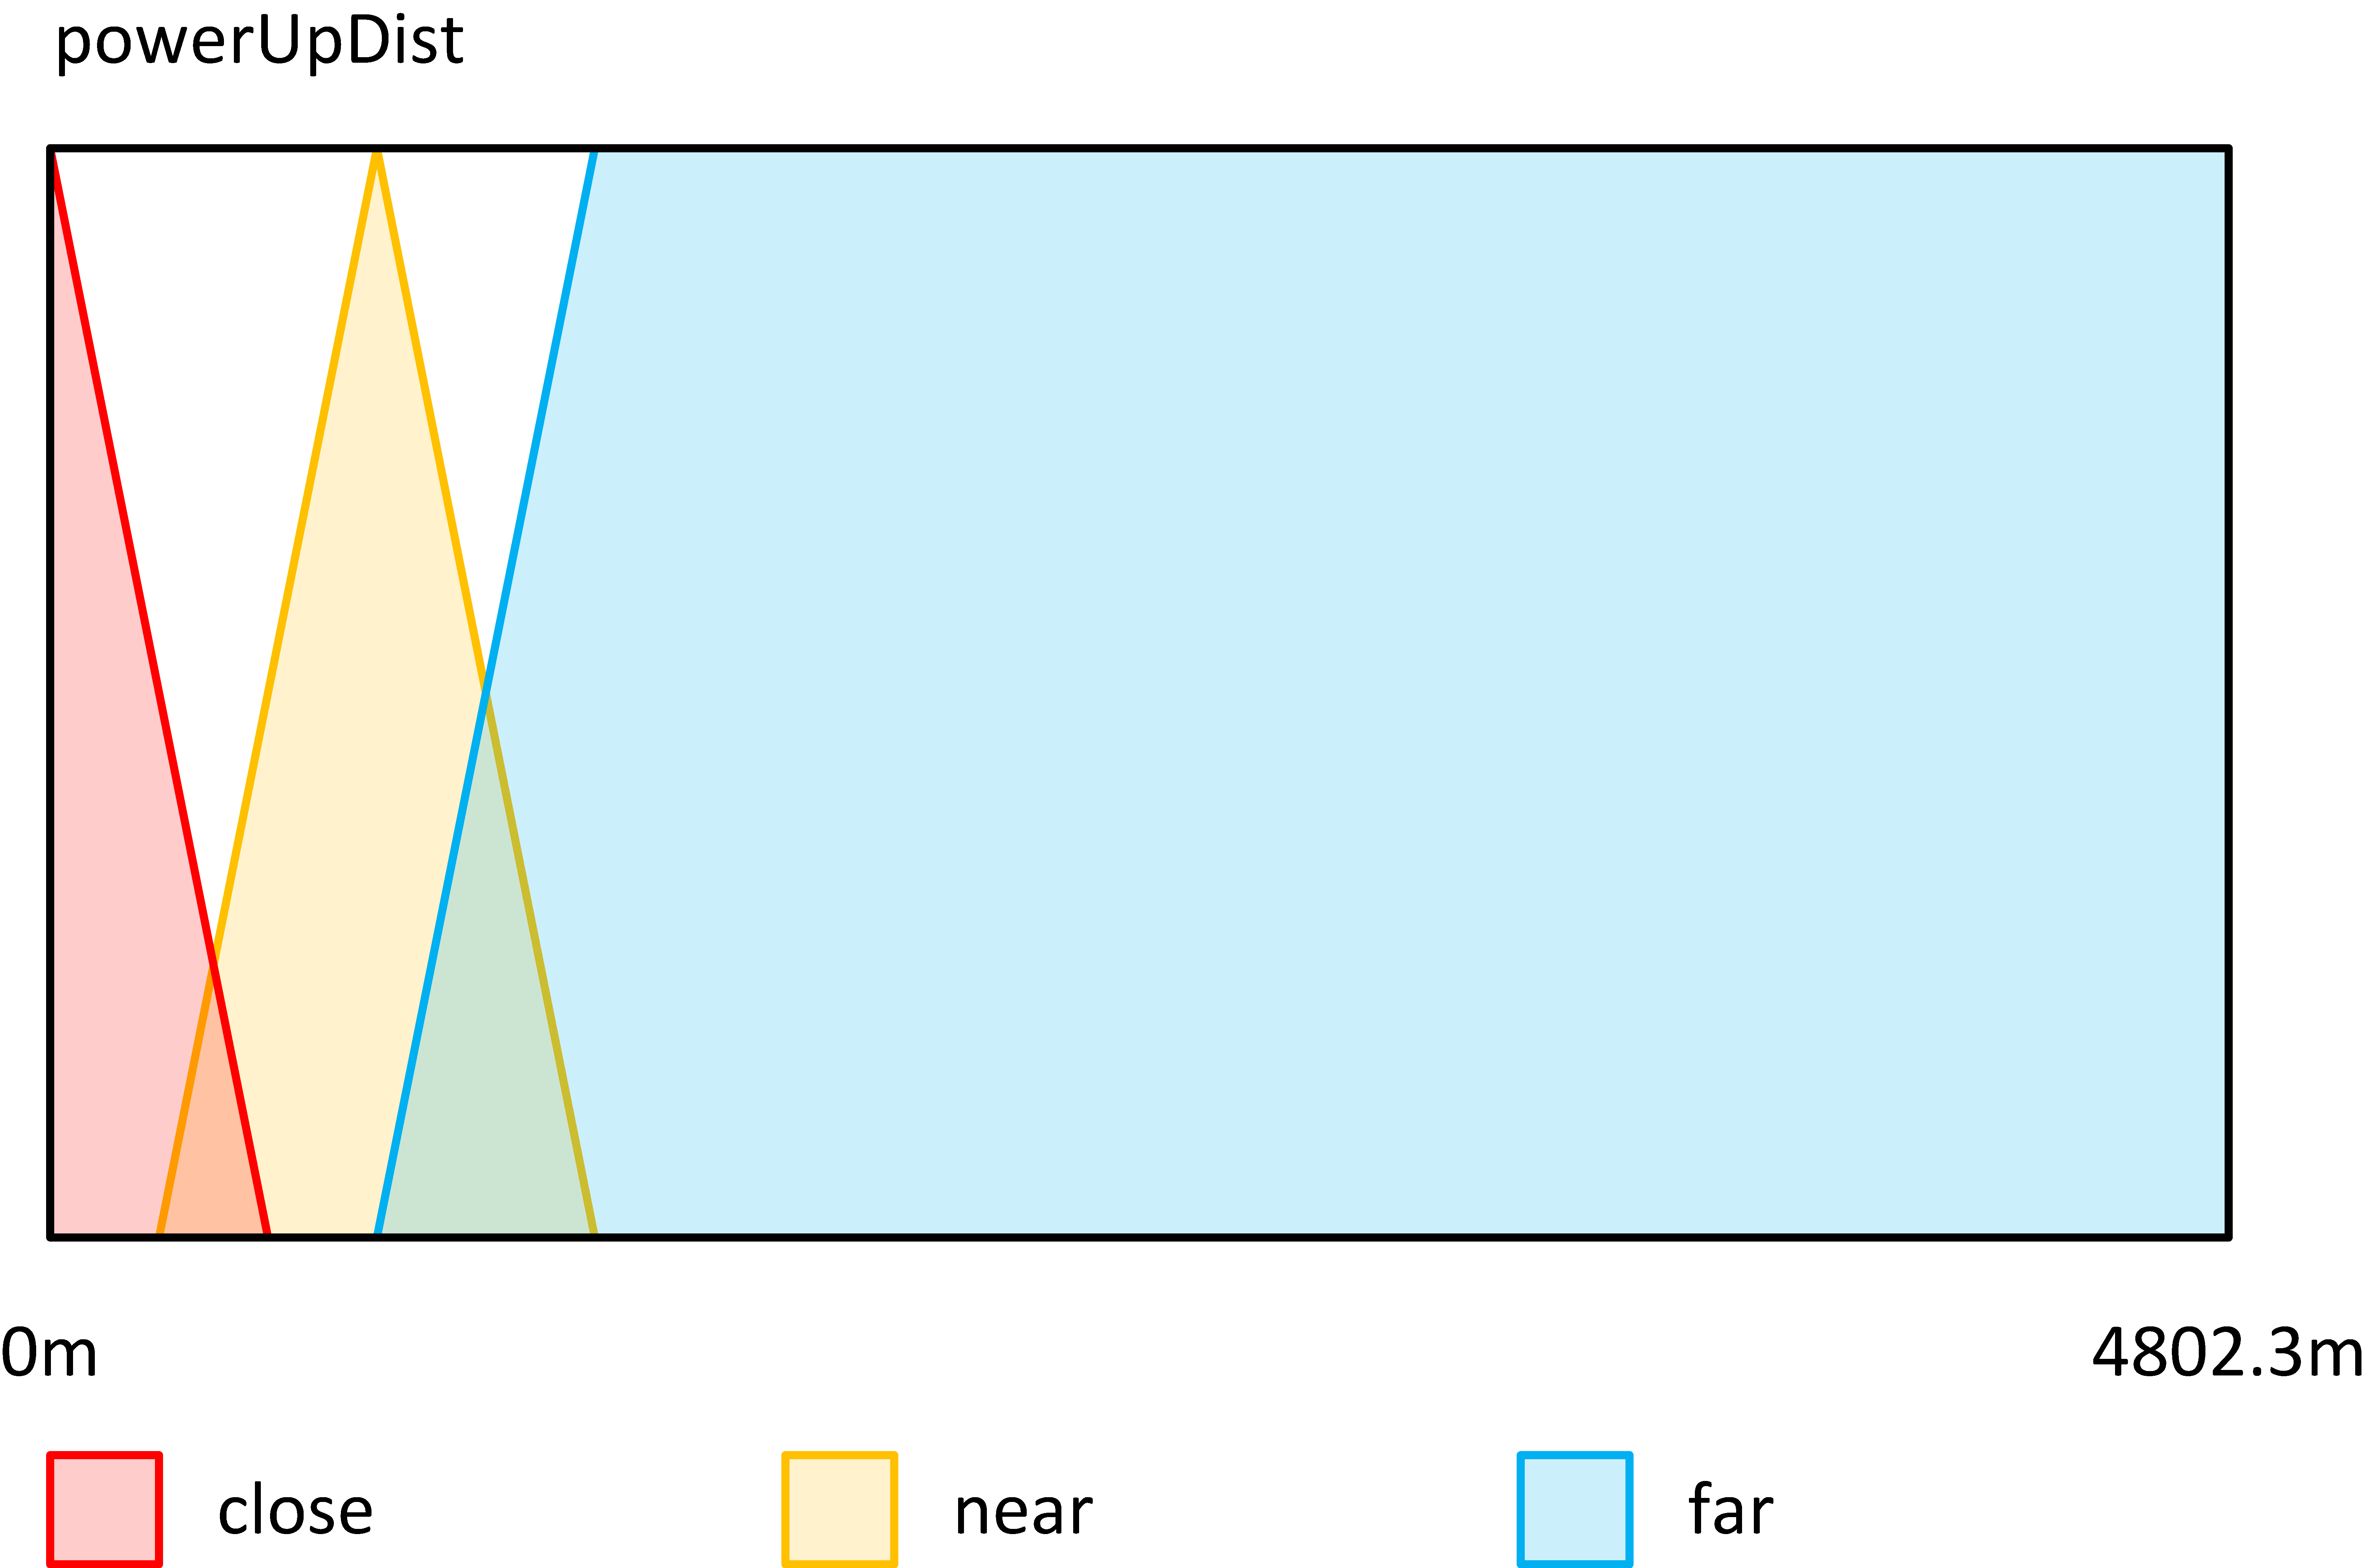
\includegraphics[scale=0.08]{./img/pdf/powerUpDistSets.pdf}
\end{figure}

\subsubsection{powerUpAspect}

The linguistic variable \emph{powerUpAspect} is the direction of the powerup in relation to the player. Again, the clock analogy has been used to determine the fuzzy sets. However, the angle-off of the powerup is not considered, since it is stationary and does not change its heading.

\begin{figure}[H]
\centering
\caption{\emph{powerUpAspect} fuzzy sets}
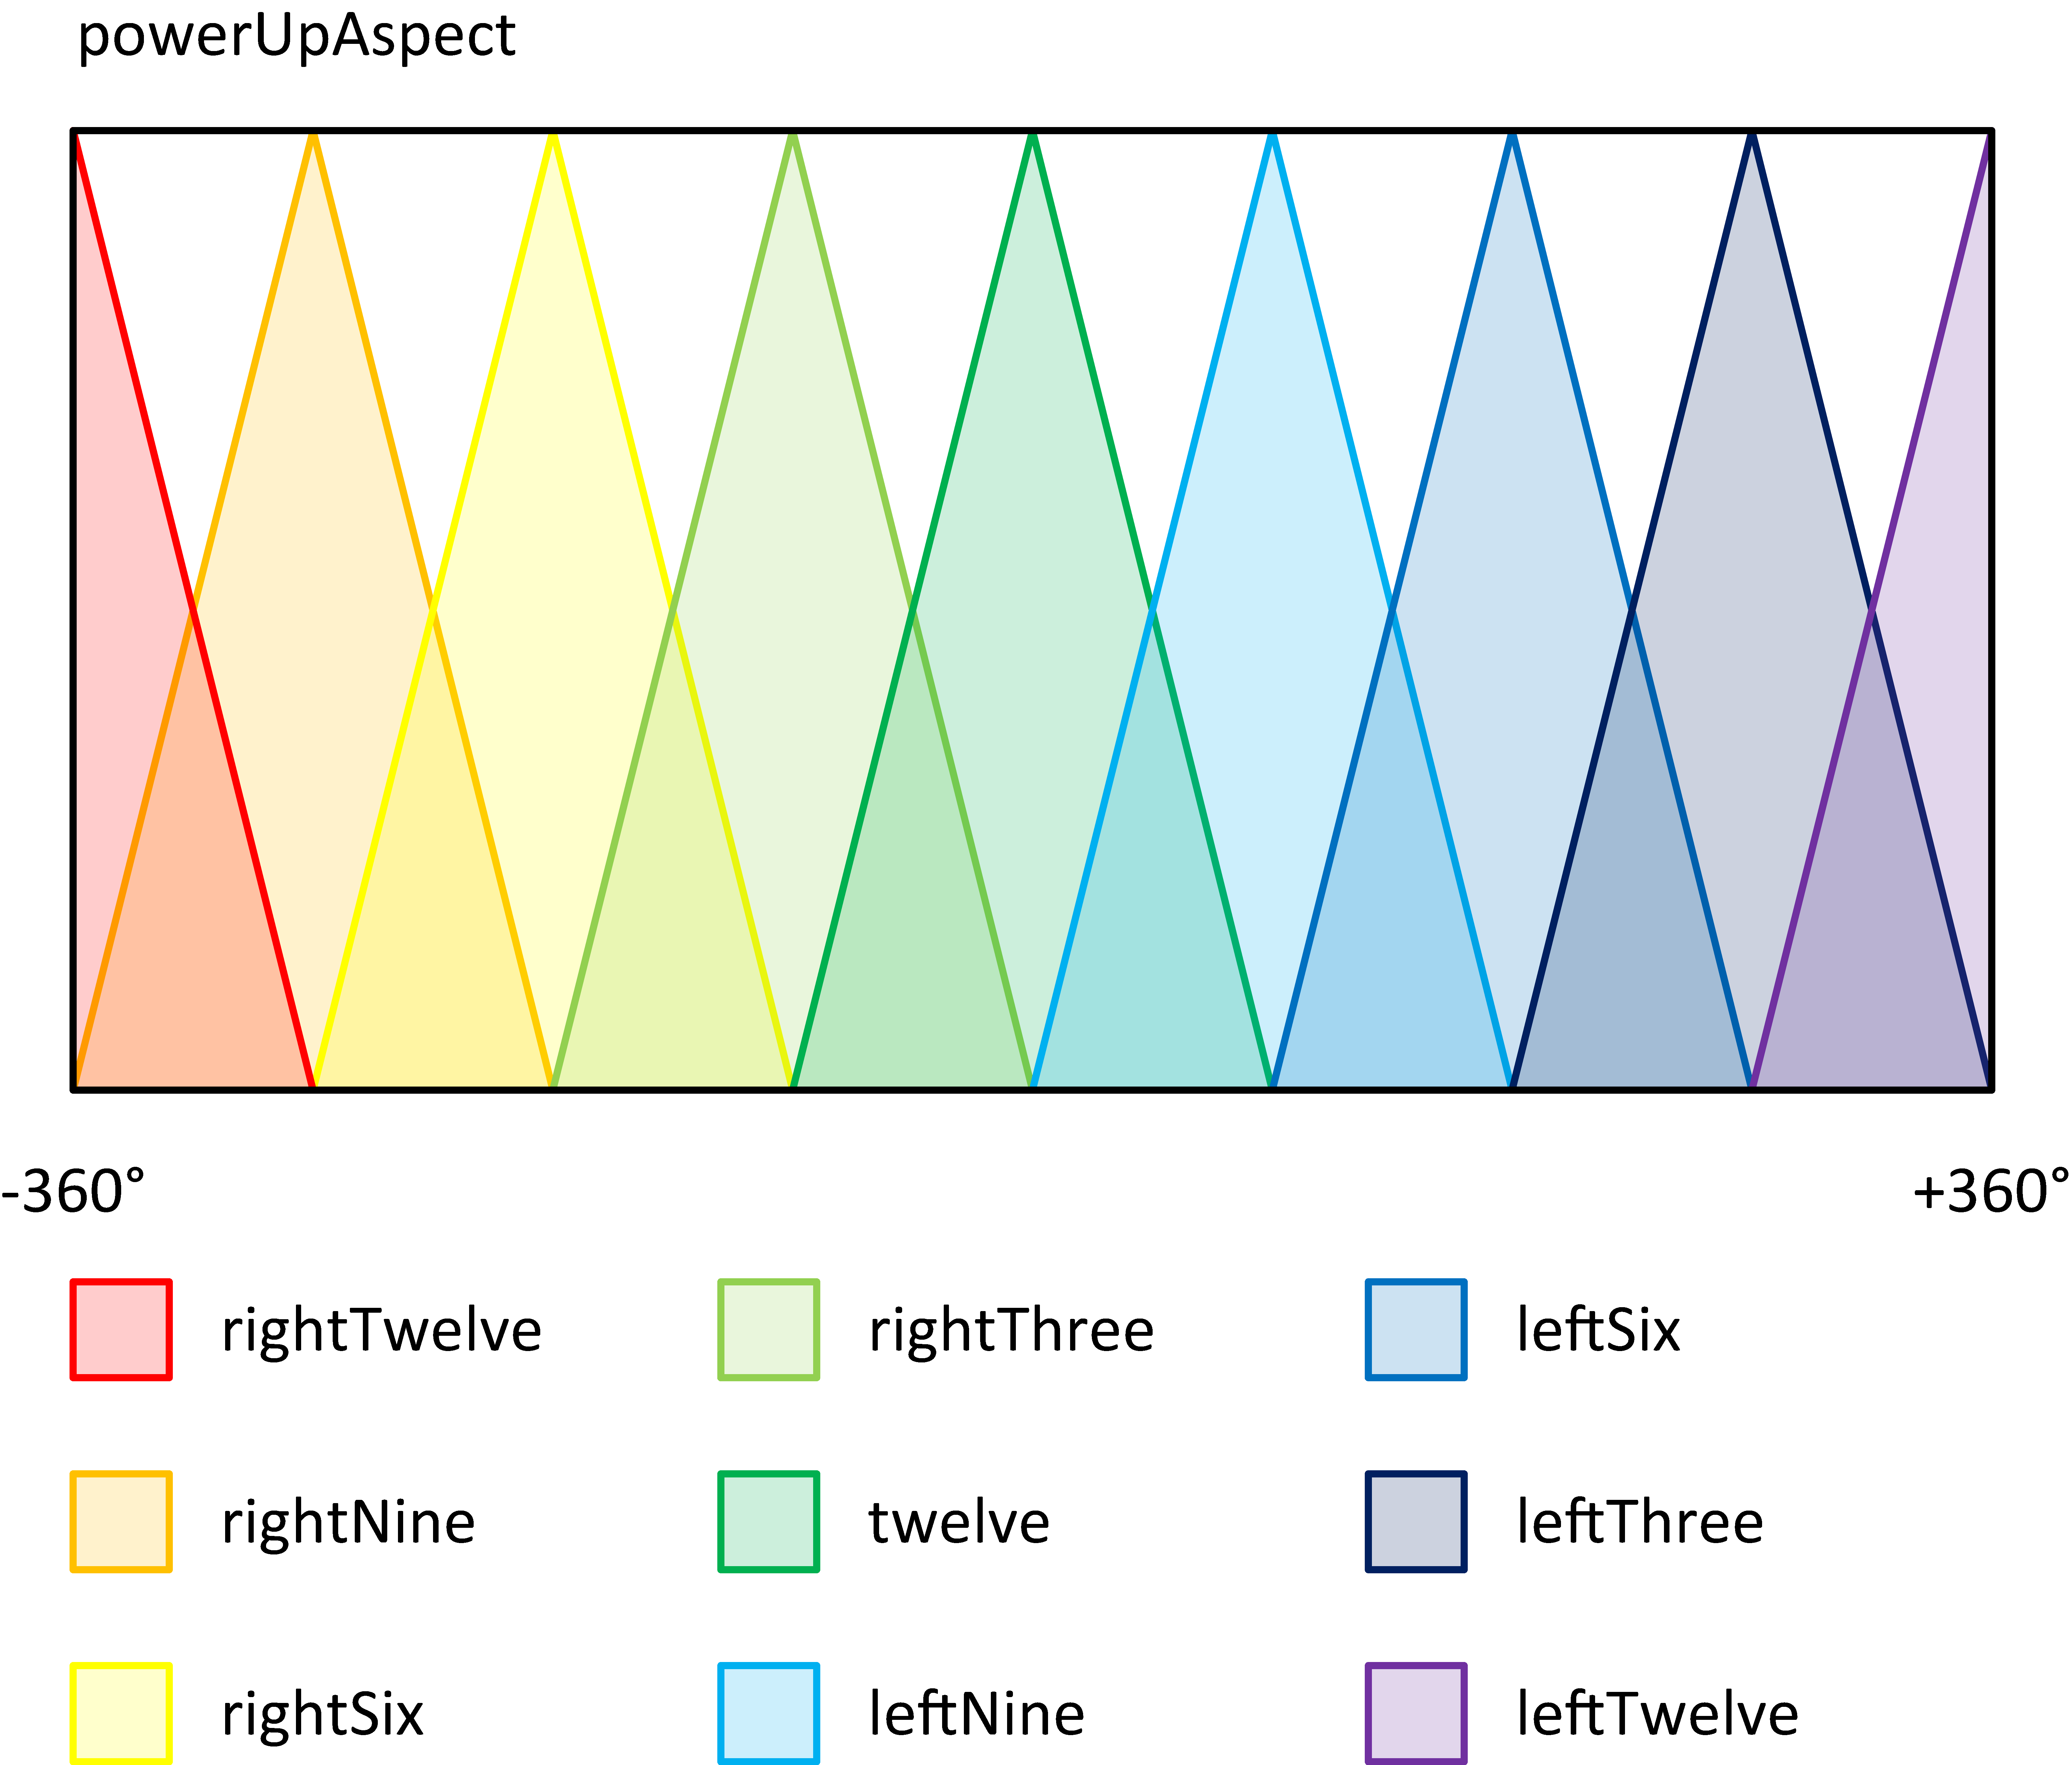
\includegraphics[scale=0.08]{./img/pdf/powerUpAspectSets.pdf}
\end{figure}

\section{Output linguistic variables}

Due to the fact that the fuzzy logic API does not provide a method to prioritize rules, defensive and offensive versions of some output linguistic variables have been defined. Boolean variables are defined, which are then tested to determine which version of the rule is fired, during a given situation.

For example, the defensive turn rule only considers the blast linguistic variables as input, whereas the offensive turn rule considers both target and blast linguistic variables.

\subsection{Defensive rules}

\subsubsection{defensiveTurn}

The \emph{defensiveTurn} linguistic variable defines which heading the saucer will take, in degrees, according to the rules that govern defensive turning. The linguistic variables used as input for \emph{defensiveTurn} are: \mintinline{console}{layerVar = blastDist}, \\ \mintinline{console}{rowVar = blastAngleOff}, and \mintinline{console}{colVar = blastAspect}, creating a 3D rule matrix. Note that \emph{r} and \emph{l} represent right and left in the table.
\\
\\
For example: IF (close) AND (rightSix) AND (zero) THEN (-90) \\
In other words, IF the energy blast is close, AND it is behind the player, AND it's heading towards the player, THEN turn right for 90$^{\circ}$.

\begin{table}[H]
\centering
\caption{\emph{defensiveTurn} \emph{close}}
\label{Turn rule table}
\begin{tabular}{r|r|r|r|r|r|r|r|r|r}
 		& rTwelve 	& rNine 	& rSix 		& rThree 		& twelve 	& lNine 	& lSix 		& lThree	& lTwelve		\\ \hline
rZero	& 0			& 0			& -90		& 0 		 	& 0			& 0			& +90	 	& 0			& 0				\\
r270	& +90		& 0			& 0			& +180			& +90		& 0			& 0			& +180		& +90			\\
rMerge	& 0			& 0			& -90	 	& 0				& 0			& 0			& +90		& 0			& 0				\\
r90		& +90		& -180		& 0 		& 0				& -90		& -180		& 0			& 0			& +90			\\
zero 	& 0			& 0 		& -90 		& 0				& 0			& 0			& +90		& 0			& 0				\\
l90 	& -90		& 0 		& 0			& +180			& +90		& 0			& 0			& +180		& -90			\\
lMerge	& 0			& 0 		& -90 		& 0				& 0			& 0			& +90		& 0			& 0				\\
l270 	& -90		& -180 		& 0			& 0				& -90		& -180		& 0			& 0			& -90			\\
lZero 	& 0			& 0 		& -90	 	& 0				& 0			& 0  		& +90		& 0			& 0				\\
\end{tabular}
\end{table}

\begin{table}[H]
\centering
\caption{\emph{defensiveTurn} \emph{far}}
\label{Turn rule table}
\begin{tabular}{r|r|r|r|r|r|r|r|r|r}
 		& rTwelve 	& rNine 	& rSix 		& rThree 	& twelve 	& lNine 	& lSix 		& lThree	& lTwelve	\\ \hline
rZero	& 0			& 0			& 0			& 0 	 	& 0			& 0			& 0	 		& 0			& 0			\\
r270	& 0			& 0			& 0			& 0			& 0			& 0			& 0			& 0			& 0			\\
rMerge	& 0			& 0			& 0	 		& 0			& 0			& 0			& 0			& 0			& 0			\\
r90		& 0			& 0			& 0 		& 0			& 0			& 0			& 0			& 0			& 0			\\
zero 	& 0			& 0 		& 0	 		& 0			& 0			& 0			& 0			& 0			& 0			\\
l90 	& 0			& 0 		& 0			& 0			& 0			& 0			& 0			& 0			& 0			\\
lMerge	& 0			& 0 		& 0	 		& 0			& 0			& 0			& 0			& 0			& 0			\\
l270 	& 0			& 0	 		& 0 		& 0			& 0			& 0			& 0			& 0			& 0			\\
lZero 	& 0			& 0 		& 0	 		& 0			& 0			& 0  		& 0			& 0			& 0			\\
\end{tabular}
\end{table}

The far rules have zero values so that the player does not react and maintains current heading when the energy blast is far, and is not a threat.

\subsubsection{defensiveSpeed}

The \emph{defensiveSpeed} linguistic variable defines how fast the saucer will travel, according to the rules that govern defensive speed. The linguistic variables used for input for \emph{defensiveSpeed} are: \mintinline{console}{layerVar = blastDist}, \mintinline{console}{rowVar = blastAngleOff}, and \mintinline{console}{colVar = blastAspect}, creating a 3D rule matrix.
\\
\\
For example: IF (close) AND (rightSix) AND (zero) THEN (125) \\
In other words, IF the energy blast is close, AND it is behind the player, AND it's heading towards the player, THEN speed is 125.

\begin{table}[H]
\centering
\caption{\emph{defensiveSpeed} \emph{close}}
\label{Turn rule table}
\begin{tabular}{r|r|r|r|r|r|r|r|r|r}
 		& rTwelve 	& rNine 	& rSix 		& rThree 		& twelve 	& lNine 	& lSix 		& lThree	& lTwelve		\\ \hline
rZero	& 50		& 125		& 125		& 125 		 	& 50		& 125		& 125 		& 125		& 50			\\
r270	& 50		& 125		& 50		& 125			& 50		& 125		& 50		& 125		& 50			\\
rMerge	& 50		& 125		& 50	 	& 125			& 125		& 125		& 50		& 125		& 50			\\
r90		& 50		& 125		& 50 		& 125			& 125		& 125		& 50		& 125		& 50			\\
zero 	& 50		& 125 		& 125 		& 125			& 50		& 125		& 125		& 125		& 50			\\
l90 	& 50		& 125 		& 50		& 125			& 125		& 125		& 50		& 125		& 50			\\
lMerge	& 50		& 125 		& 50	 	& 125			& 125		& 125		& 50		& 125		& 50			\\
l270 	& 50		& 125	 	& 50 		& 125			& 50		& 125		& 50		& 125		& 50			\\
lZero 	& 50		& 125 		& 125	 	& 125			& 50		& 125  		& 125		& 125		& 50			\\
\end{tabular}
\end{table}

\begin{table}[H]
\centering
\caption{\emph{defensiveSpeed} \emph{far}}
\label{Turn rule table}
\begin{tabular}{r|r|r|r|r|r|r|r|r|r}
 		& rTwelve 	& rNine 	& rSix 		& rThree 		& twelve 	& lNine 	& lSix 		& lThree	& lTwelve		\\ \hline
rZero	& 50		& 50		& 75		& 50 		 	& 50		& 50		& 75 		& 50		& 50			\\
r270	& 50		& 50		& 50		& 75			& 50		& 50		& 50		& 75		& 50			\\
rMerge	& 50		& 50		& 50	 	& 50			& 75		& 50		& 50		& 50		& 50			\\
r90		& 50		& 75		& 50 		& 50			& 75		& 75		& 50		& 50		& 50			\\
zero 	& 50		& 50 		& 75 		& 50			& 50		& 50		& 75		& 50		& 50			\\
l90 	& 50		& 50 		& 50		& 75			& 75		& 50		& 50		& 75		& 50			\\
lMerge	& 50		& 50 		& 50	 	& 50			& 75		& 50		& 50		& 50		& 50			\\
l270 	& 50		& 75	 	& 50 		& 50			& 50		& 75		& 50		& 50		& 50			\\
lZero 	& 50		& 50 		& 75	 	& 50			& 50		& 50  		& 75		& 50		& 50			\\
\end{tabular}
\end{table}

\subsection{Offensive rules}

\subsection{Neutral}

\subsubsection{getPowerTurn}


\section{Learnings}

Due to the greater amount of input sensors provided, this controller is vastly different to the one submitted with the first assignment. It is now possible to define rules with higher complexity, and therefore 3D rule matrices are a necessity. The larger player count also requires a completely different strategy. In the first assignment, the main strategy was to be aggressive from the start. In comparison, this controller needs to be much more defensive and aim to survive until the end of the battle.

With that in mind, I began with blast sensor inputs. Rather than attempt to implement multiple sensors at once, I was able to focus on the controller's performance on dodging energy blasts and developed a well-performing ruleset just for turning. Experience from the first assignment assisted in defining controlled turn rules, resulting in less erratic movement. I reused the clock analogy for target/blast/powerup directions, and also considered the heading of moving objects to decide which direction to turn the player. 

However, I came across an issue where the controller would switch between -180 and +180 when an energy blast was behind the player. Rules dictated that the player would turn either left or right, depending on if the energy blast position was a positive or negative number. Because the sensor value was switching between positive and negative values erratically, the controller also flicked between left and right turns, resulting in the player not turning at all, and continued to move straight and was always hit by energy blasts from behind. To remedy this, I decided to stick to a single direction of turn, which in this case was a right hand 90$^{\circ}$ turn. This resolved the issue and the player now dodges energy blasts very well from the 6 o'clock position, albiet only in right hand turns.

I encountered an issue where I wished to prioritize turn rules that tell the player to move directly to a powerup over turn rules that dodge energy blasts. I emailed the tutor, Philip Hingston, who advised me that this was not possible. The alternative was to set up a combination of fuzzy and if-then rules. I implemented this concept and realised this opened up other possibilities for rules, as seen with the defensive and offensive versions of my output variables. I found similarities in this concept with the Tartarus problem of Workshop 7, which assisted in designing the if-then rules. I can see the potential that if-then statements have in developing richer, more complex rules.

The controller has potential to be improved. For example, firepower rules could utilize target heading, and only fire if the target is facing the player. I observe that the player can sometimes waste shots if the target is running away and does a good job at dodging energy blasts. The turn rules also have room for improvement. There are some situations where the player makes a wrong turn, or does not react quick enough to an incoming energy blast. I am pleased with the powerup strategy I have implemented, as it ignores energy blasts and suppresses enemies nearby while heading straight for the powerup. However, there are cases where the nearest enemy to the player is not the one closest to the powerup, and energy is wasted firing at the maximum rate. This could be improved by determining which enemy is closest to the powerup and firing at it, or by having the ability to fire at the powerup directly.
\section{Conclusion}

This report examined the application of fuzzy logic using Sugeno style inference in a video game. The video game involved developing a fuzzy logic controller, which controls an armed flying saucer with a goal of surviving the battle as the last one standing by the end of the battle.

The linguistic input variables and their fuzzy sets were explored, as well as the output variables and associated rules. Rule overrides were also explained. These rules governed the behaviour of the saucer and attempted to implement the overall strategy developed for this assignment:

\begin{itemize}
\item Fly defensively
	\begin{itemize}
	\item Conserve energy
	\item Keep rate of fire to a minimum
	\item Focus movement on dodging energy blasts
	\end{itemize}
\item If a powerup spawns nearby
	\begin{itemize}
	\item Stop dodging energy blasts
	\item Move straight to the powerup at high speed
	\item If there are no close, incoming energy blasts, fire at maximum rate of fire to deter others from reaching the powerup
	\item If there are close, incoming energy blasts, deploy shield
	\end{itemize}
\item If there are only two enemies left
	\begin{itemize}
	\item React to any powerup, even those that are far, to starve the remaining enemies of extra power
	\item Fly aggressively
	\item Increase rate of fire
	\item Attempt to destroy remaining enemies before timer runs out
	\end{itemize}
\end{itemize}

\subsection{Results}

The following tables display the results of tournaments between \emph{royalRumble} vs. \emph{simple} and \emph{sitting duck} controllers, as well as \emph{royalRumble} vs. all \emph{simple} controller opponents.

\begin{table}[H]
\centering
\caption{\emph{royalRumble} vs. \emph{simple} and \emph{sitting ducks}}
\label{checkSix vs. simple}
\begin{tabular}{r|r|r|r|r|r|r|r|r|r|r|r}
Controller	& 1	 & 2  & 3  & 4  & 5  & 6  & 7  & 8  & 9  & 10 & Avg \\ \hline
royalRumble & 2	 & 2  &	1  & 1  & 1  & 1  & 1  & 1  & 2  & 1  & 1.3 \\
simple		& 4	 & 11 &	7  & 2  & 6  & 6  & 2  & 10 & 10 & 9  & 6.2 \\
simple		& 5	 & 1  &	3  & 5  & 2  & 3  & 3  & 11 & 11 & 2  & 3.7 \\
simple		& 3	 & 6  &	9  & 3  & 3  & 5  & 6  & 1  & 1  & 5  & 4.4 \\
simple		& 10 & 4  & 2  & 10 & 4  & 2  & 8  & 9  & 9  & 7  & 6.0 \\
simple		& 6  & 5  & 4  & 6  & 5  & 4  & 10 & 4  & 4  & 4  & 5.9 \\
duck		& 9  & 9  & 8  & 4  & 11 & 9  & 5  & 8  & 5  & 12 & 8.0 \\
duck		& 11 & 8  & 5  & 9  & 12 & 11 & 11 & 12 & 8  & 6  & 9.3 \\
duck		& 8  & 10 & 10 & 8  & 9  & 12 & 4  & 7  & 3  & 8  & 7.9 \\
duck		& 12 & 3  & 6  & 12 & 8  & 10 & 12 & 6  & 12 & 3  & 8.4 \\
duck		& 7  & 12 & 11 & 11 & 7  & 7  & 9  & 9  & 7  & 10 & 9.0 \\
duck		& 2  & 7  & 12 & 7  & 10 & 8  & 7  & 10 & 6  & 11 & 8.0
\end{tabular}
\end{table}

\begin{table}[H]
\centering
\caption{\emph{royalRumble} vs. \emph{simple}}
\label{checkSix vs. simple}
\begin{tabular}{r|r|r|r|r|r|r|r|r|r|r|r}
Controller	& 1	 & 2  & 3  & 4  & 5  & 6  & 7  & 8  & 9  & 10 & Avg \\ \hline
royalRumble & 2	 & 2  &	1  & 1  & 2  & 1  & 1  & 2  & 2  & 1  & 1.5 \\
simple		& 7	 & 2  &	3  & 4  & 4  & 12 & 9  & 3  & 12 & 2  & 5.8 \\
simple		& 4	 & 3  &	2  & 5  & 12 & 9  & 8  & 9  & 1  & 10 & 6.3 \\
simple		& 3	 & 4  &	4  & 3  & 9  & 7  & 10 & 4  & 8  & 8  & 6.0 \\
simple		& 10 & 8  & 10 & 7  & 7  & 2  & 4  & 5  & 3  & 5  & 6.1 \\
simple		& 11 & 6  & 7  & 10 & 11 & 5  & 7  & 12 & 11 & 12 & 9.2 \\
simple		& 1  & 12 & 11 & 2  & 5  & 8  & 11 & 8  & 7  & 3  & 6.8 \\
simple		& 9  & 10 & 12 & 11 & 8  & 10 & 6  & 7  & 6  & 11 & 9.0 \\
simple		& 8  & 5  & 5  & 9  & 10 & 3  & 3  & 1  & 5  & 6  & 5.5 \\
simple		& 5  & 9  & 9  & 8  & 6  & 6  & 2  & 11 & 10 & 7  & 7.3 \\
simple		& 6  & 7  & 8  & 12 & 3  & 11 & 12 & 10 & 4  & 9  & 8.2 \\
simple		& 12 & 11 & 6  & 6  & 1  & 4  & 5  & 6  & 9  & 4  & 6.4
\end{tabular}
\end{table}

%\newpage
%\urlstyle{rm}
%\bibliographystyle{apacite}
%\addcontentsline{toc}{section}{References}
%\bibliography{./bib/Year_2-Sem_1-CSG2341-0b_A1}


\end{document}